\documentclass[a4paper,8pt]{report}
\usepackage{graphicx}
\usepackage{epsfig}
%opening
\title{Decentralized time(frame) Synchronization Algorithm for a Distributed Wireless Sensor Network}
\author{Fasika A.Assegei}
\begin{document}
\maketitle
\newpage
\begin{abstract}
Time synchronization is a crucial component of infrastructure for
wireless sensor networks (WSN). Most applications of WSNs make
extensive use of time synchronization like TDMA scheduling, accurate
timestamping of events, coordinate activities of the network or data
fusion. The unique requirements of wireless sensor networks in terms
of precision, lifetime, energy and scope of the synchronization
achieved, make the traditional synchronization methods unsuitable
for WSNs. This inspires for the need of synchronization methods for
WSNs which are aligned to the specific properties of WSN. In this
thesis, different algorithms are developed to achieve a stable,
convergent and energy-efficient synchronization of a decentralized
WSN. The algorithms achieve synchronization by using the phase
offset of a node's wakeup time with that of the neighboring node's,
without actually exchanging the information about the clock time of
the sender. So, the method avoids time keeping on the messages(time
stamping) which reduces the message overload. The algorithm can be
integrated with the slot allocation algorithm to form the Mac layer
protocol for a better throughput. At the end of the thesis, the
comparison of the algorithms in terms of energy consumption is
presented. A low energy-consumption or a better convergence as well
as the length of the guard time can be used to select the proper
algorithm for different applications.
\end{abstract}
\newpage
\tableofcontents
\newpage
\newpage
\listoffigures
\newpage
\chapter{Introduction}
\section{Wireless Sensor Networks} Technological advances have led
to the development of low-cost sensors, which are capable of
wireless communication and data processing. Wireless sensor
networks(WSNs) are distributed networks of such sensors, dedicated
to closely observing real-world phenomena. Such sensors may be
embedded in the environment  or enabled with mobility;they can be
deployed in inaccessible, dangerous, or hostile environments. The
sensors need to configure themselves in a communication network, in
order to collect information that has to be pieced together to
assemble a broader picture of the environment than what each sensor
individually senses. Diverse applications are realized using sensor
networks$\cite{9}$. Thus, as the WSNs become an integral part of the
modern era, addressing issues in designing such networks become
necessary.
\newline One of the design issues in WSNs is clock
synchronization. Clock synchronization is a critical piece of
infrastructure in any distributed system. In sensor networks, a
number of factors makes flexible and robust time synchronization
particularly important, while simultaneously making it more
difficult to achieve than in traditional networks.
\newline
Collaboration among nodes is often required for different purposes.
A common view of physical time is a basic requirement for nodes to
reason about events that occur in the physical world. In addition to
these domain-specific requirements, sensor network applications
often rely on synchronization as typical distributed systems do: for
a proper TDMA scheduling, for database queries, cryptography and
authentication schemes, coordination of future action, interaction
with users, ordering logged events during system debugging, and so
forth.\newline \textbf{Unnecessary synchronization wastes resources;
insufficient synchronization leads to poor application performance.
}\newpage
\section{Existing Work on WSN clock synchronization}
      Several algorithms have been proposed and researched for time synchronization in
sensor networks.
      The reference broadcast synchronization (RBS) designed by $\ref{f}$ is an important
scheme in the area of WSN synchronization. It achieves a R-R
pairwise synchronization to remove sender nondeterminism and results
in a good precision of a few microseconds. It also provides
frequency estimates between two receivers using a linear regression
technique. But the message overhead is very large. $\cite{12}$
presents a decentralized slot allocation algorithm based for TDMA
networks which uses the topology of the nodes as a means to weigh
the offset of the node. The message has the overhead due to the
transfer of the topology distance identifier.
      A probabilistic method of clock synchronization is described in $\cite{1}$. The authors
extend a deterministic protocol like RBS to provide bounds on the
accuracy of clock synchronization, and provide protocol parameters
to make it adaptive by making provision for tradeoff between
accuracy and protocol parameters.
      $\cite{1}$ suggests a mathematical approach which leads to a protocol that provides optimal
       synchronization in a very high density of nodes. They derive an optimal estimator for
determining the state of an ideal nodes clock and thus provide a
global synchronization in which all the nodes are synchronized
optimally with the sender.
      Another method for achieving a network-wide synchronization is suggested by $\ref{}$.
This approach first establishes a hierarchical structure and then
performs a pairwise synchronization along its edges, resulting in a
good accuracy which does not degrade over multihop. The algorithm
suggested by [10] also achieves a lightweight, multihop
synchronization in a similar tree-based scenario.
      In situations where temporal ordering of events matter more than absolute time of
occurrence, the scheme suggested by [12], for sparse sensor
networks, provides a modest synchronization. It gives mapping of
intervals between events from clock readings made on one node to thewith
clocks of other nodes, without trying to synchronize with a common
time-base. Though this scheme has very little overhead, it provides
a localized and instantaneous synchronization with only 1 ms
accuracy. An improved version of this interval method is proposed by
[13] which provides the worst and best case of achievable time
uncertainty in an ad-hoc sensor networks scenario.
      An interesting method suggested by [14] presents an adaptive
protocol, which along with providing a good accuracy, adapts itself
to the environmental conditions and user- defined precision by adjusting
the sampling rate, thus avoiding any wastage of energy.
      It can be observed that these time synchronization approaches
suggested for sensor networks fall into many separate points in the parameter space
described in previous section. Each of these schemes have trade-offs
and no single method is yet optimal on all axes. Another approach is
used in $f$ to use the metaphor of fireflies to the existing problem
of synchronization which bases itself in the synchronization of the
network which is focused on the same domain. \newline In $[]$, the
synchronization of the network is studied where convergence is
acheived for a network of nodes in a decentralized manner.
\section{Objective and overview of the thesis}
      There are many schemes presented to provide time synchronization
for the warless sensor networks. It was observed that most of the
schemes use a central node in order to achieve a synchronization
with the nodes. In addition, most methods are used to build a table
corresponding the clock of the sender and the receiver using
timestamping. It therefore applies only to a set of applications and
a lot of energy will be spent if nodes need to be synchronized
often. Also, if the nodes are subjected to severe changes in
environmental conditions, then the accuracy of these short-term
synchronization schemes might suffer a lot.
\newline
The primary objective of the thesis is to develop an algorithm to
achieve a long time synchronization of a distributed WSN in a low
cost and energy-efficient method. This decentralized approach
results in an efficient method concerning the energy of the WSN. The
methods use the phase offset between the sender and receiver,
without actually taking the senders clock a way of achieving
long-term time synchronization in sensor networks. Here, there are
three algorithms present to achieve a long term synchronization of a
distributed WSN. A comparison is made and the results are presented.
Thus a protocol can be built around these algorithms, in integration
with the slot allocation algorithm to be incorporated in the MAC
layer protocol. This protocol is able to achieve a long- term time
synchronization that has the following characteristics: provides
high precision, adaptive to environmental effects, energy-efficient,
scalable..
\newline The remainder of the thesis is organized as follows:  Chapter 2
presents a general overview of synchronization in WSN and the need
for a synchronized time. Chapter 3 discusses the synchronization
error and formulate the problem. Chapter 4 presents the mathematical
models of the algorithms for the synchronization of the network. In
Chapter 5 we present the computer simulation results and the
analysis of the results in addition to the comparison of the three
methods with respect to the energy consumption. Finally, Chapter 7
draws the conclusions from this thesis and suggests some future
work.
\newpage
\chapter{Synchronization in Wireless Sensor Networks}
\section{Introduction}Chess$\footnote{Chess specialises
in innovative technical systems and business critical solutions.
Chess creates and develops sophisticated solutions and products for
electronic systems, transactions and electronic payments, Machine to
Machine (M2M) systems, sensor applications and digital multimedia.
Chess is located in Haarlem, the Netherlands.}$ created a MAC
protocol, G-MAC, with the gossiping technique in mind. A separate
research is being conducted on the MAC protocol at Chess B.V. As a
sensor network, the duty cycle of the network is small, around
1$\%$. Looking back at the 1$\%$ active time versus the $99\%$
nonactive time ratio, it is a non-trivial matter to keep the nodes
synchronized. A number of approaches have been introduced, of which
carrier sense multiple access (CSMA) and time division multiple
access (TDMA) are the most common. One problem with CSMA is the
times when the radio is busy with idle listening. Nodes need to
listen to the radio for periods of time before they can actually
send data. In TDMA, time is divided into discrete slots. Nodes
transmit in rapid succession in one time-slot and listen in the
others. To reduce the idle listening even more, the listening nodes
can turn off the radio for the time between the end of the
transmission and the start of a new slot. In theory, there will not
be any idle listening. There are some pitfalls to this approach. As
mentioned before, the clocks of the nodes are less than perfect;
they will never run at the same clock-speed. To keep the nodes
synchronized and thus to let them share the same schedule, the small
timing error needs to be compensated. Second, there has to be a
certain algorithm to allocate the slots among the nodes; they cannot
simply all start broadcasting in the first slot, since that would
cause nothing but collisions. The research on slot allocation
algorithm is being conducted alongside this research.
\section{Clock Synchronization in traditional networks}
In a centralized system the solution to clock drift is trivial: the
centralized server will dictate the system time because time is
unambiguous. When a process wants to know the time, it makes a
system call and the kernel tells it. If process A asks for the time,
and then a little later process B asks for the time, the value that
B gets will certainly be higher than the value A got$\cite{1}$. With
this centralized concept in mind, different protocols have been
proposed and implemented to achieve synchronization in traditional
networks, Network Time Protocol(NTP) being the most popular.
\newline
Infrastructure advantage being the most important factor, the
Network Time Protocol (NTP) is one of the most accurate and flexible
means of sending time over the Internet. The protocol is designed to
compensate for some, but not all, network time delays between the
server and the client. NTP is most successful across local area
networks and can give accuracy as good as a few milliseconds. On the
world wide web, however, time transfer delays are at the mercy of
server traffic and network bottlenecks, and accuracy figures cannot
be quoted as easily.
\newline NTP uses a round time delay to a universal time reference
 so that it can adjust the clock of the networked component NTP
 is a tiered time distribution system with redundancy capability.
 NTP measures delays within the network and within the algorithms
 on the machine on which it is running. Using
these tools and techniques, it is able to synchronize clocks to
within milliseconds of each other when connected on a Local Area
Network and within hundreds of milliseconds of each other when
connected to a Wide Area Network. The tiered nature of the NTP time
distribution tree enables a user to choose the accuracy needed by
selecting a level (stratum) within the tree for machine placement. A
time server placed higher in the tree (lower stratum number),
provides a higher likelihood of agreement with the UTC time
standard. \newline Some of the hosts act as time servers, that is,
they provide what they believe is the correct time to other hosts.
Other hosts act as clients, that is, they find out what time it is
by querying a time server. Some hosts act as both clients and time
servers, because these hosts are links in a chain over which the
correct time is forwarded from one host to the next. As part of this
chain, a host acts first as a client to get the correct time from
another host that is a time server. It then turns around and
functions as a time server when other hosts, acting as clients, send
requests to it for the correct time. Should the time server from
which NTP is synchronizing fail, NTP retains the ability to maintain
an accurate clock.\newline Synchronization in traditional
distributed systems takes a different kind of approach since there
is no central authority to be referred in case of time requests. But
central nodes can be assigned as to play the role of a server as in
the case of the centralized system.
\newline But in a distributed system, creation of a synchronization scheme that
satisfies such a broad spectrum of requirements is challenging. The
task becomes particularly daunting in sensor networks, in light of
their additional domain requirements including energy efficiency,
scalability through localized interactions, and automatic adaptation
to dynamics. These complications are startling to look for a new
arena for the synchronization of Wireless sensor networks. $Figure
and reference to NTP,$.\newpage
\section{Wireless Sensor Networks: Why different ?}
     Are traditional time-synchronization methods applicable even in case of sensor networks? Many
assumptions in the traditional schemes do not hold true in the case
of WSNs $\cite{}$. Some of these factors can be described as
follows:
\begin{itemize}
\item \textbf{Energy Constraint}: Owing to their small size and nature of applications which they
      are designed for, energy is a major concern in a WSN. Classical synchronization
      algorithms are based on assumptions like, CPU is available for use most of the
      time, listening to network is free, frequent transmissions and re-transmissions are
      possible. These very factors lead to a lot of energy consumption in a sensor
      network. Thus, an energy efficient method is an appropriate
      one for wireless sensor networks.
\item \textbf{Dynamic Topology}: In a centralized system, the topology remains more or less static, and
      this fact is used by NTP for being configured. There are servers available through-
      out, which serve as a source of external time, and other nodes synchronize with
      them forming a hierarchy. Also it assumes that nodes are connected before they
      need synchronization. In a WSN, network dynamics results from various factors like
      mobility of nodes, node failures, environmental obstructions etc., which prevents
      simple static configurations. Hierarchical structures might get nodes poorly
      synchronized, and nodes might not be connected when they need synchronization the
      most.
\item \textbf{Variety of applications}: WSNs are used for a variety of applications, which can
      have totally different needs as far as synchronization is concerned. For example,
      localization applications need a short-lived but highly precise synchronization, while
      target tracking applications can tolerate a little lower precision, but want the
      synchronization to last longer. Also some applications might need a global timescale
      while some others can do only with a local timescale. And while a few require
      absolute or real time as reference, for some others, a relative notion of time is
      enough.
\item \textbf{Cost and Form factor}: Sensor nodes are very small in size and also cheap. Now,
      we can obtain very good synchronization with GPS receivers, but it will be
      unreasonable to put a $\$100$ GPS receiver on a disposable sensor
      which is costly.
\end{itemize}
All the above factors make the problem of time synchronization more
challenging in case of sensor networks. Keeping them in mind, we can
formulate some design requirements, in general, for sensor network
time synchronization:
\begin{itemize}
 \item \textbf{Energy efficient}: The energy required to achieve synchronization should be mini-
      mum as energy is the scarce resource in WSNs.
 \item \textbf{Multimodal and Tunable} The synchronization provided should be necessary
      and sufficient for the current conditions. We want the scheme
      to have a good accuracy, but at the same time save energy by not providing more
      accuracy than required. It will be best to have some parameters for tuning the
      algorithm to our requirements.
 \item \textbf{Adaptive}: The synchronization should adapt itself to the needs of application
     regarding various factors such as scope, lifetime, precision, scalability etc.
 \item \textbf{Robust to Ad-Hoc Networks}: Changes in the network topology, node mobility,
    node failure should not result in a total collapse of the synchronization architecture
    or even a drastic change in its accuracy.
 \item \textbf{Global Scale synchronization}: The algorithms should achieve a global synchronization
  which encompasses the whole network in focus.
 \item \textbf{Post-facto or Always On}:  Some applications need the nodes to synchronize
  only after an event of interest has happened, i.e. Post-Facto, and some other
  applications, like TDMA scheduling, need the nodes to be synchronized all the
  time. In our case, the nodes are required to be synchronized all the time since
  the target is for TDMA scheduling.
 \item \textbf{Relative or Absolute Time}: The synchronization algorithm should have a provision
  to provide a relative timescale within the network or get all nodes synchronized
  to absolute time, as required.
\end{itemize}
\section{The need for synchronization}
\subsection{MyriaNed}We consider that two
nodes have their TDMA schedule synchronized when the numbers of the
current time slot of any of the TDMA schedules involved are the same
for any given moment in time. The types of the slot may be
different. To successfully setup a network, the nodes has to be
synchronized and capable to send and receive messages. To establish
a link between neighboring nodes, a particular node needs to know
the schedule of all its neighbors. This can be done just sending
also the TX slot number besides the normal payload information.
Whenever a message is received, the current node acts as a slave in
relation with the transmitter, which is a master.
\begin{figure}
\centering
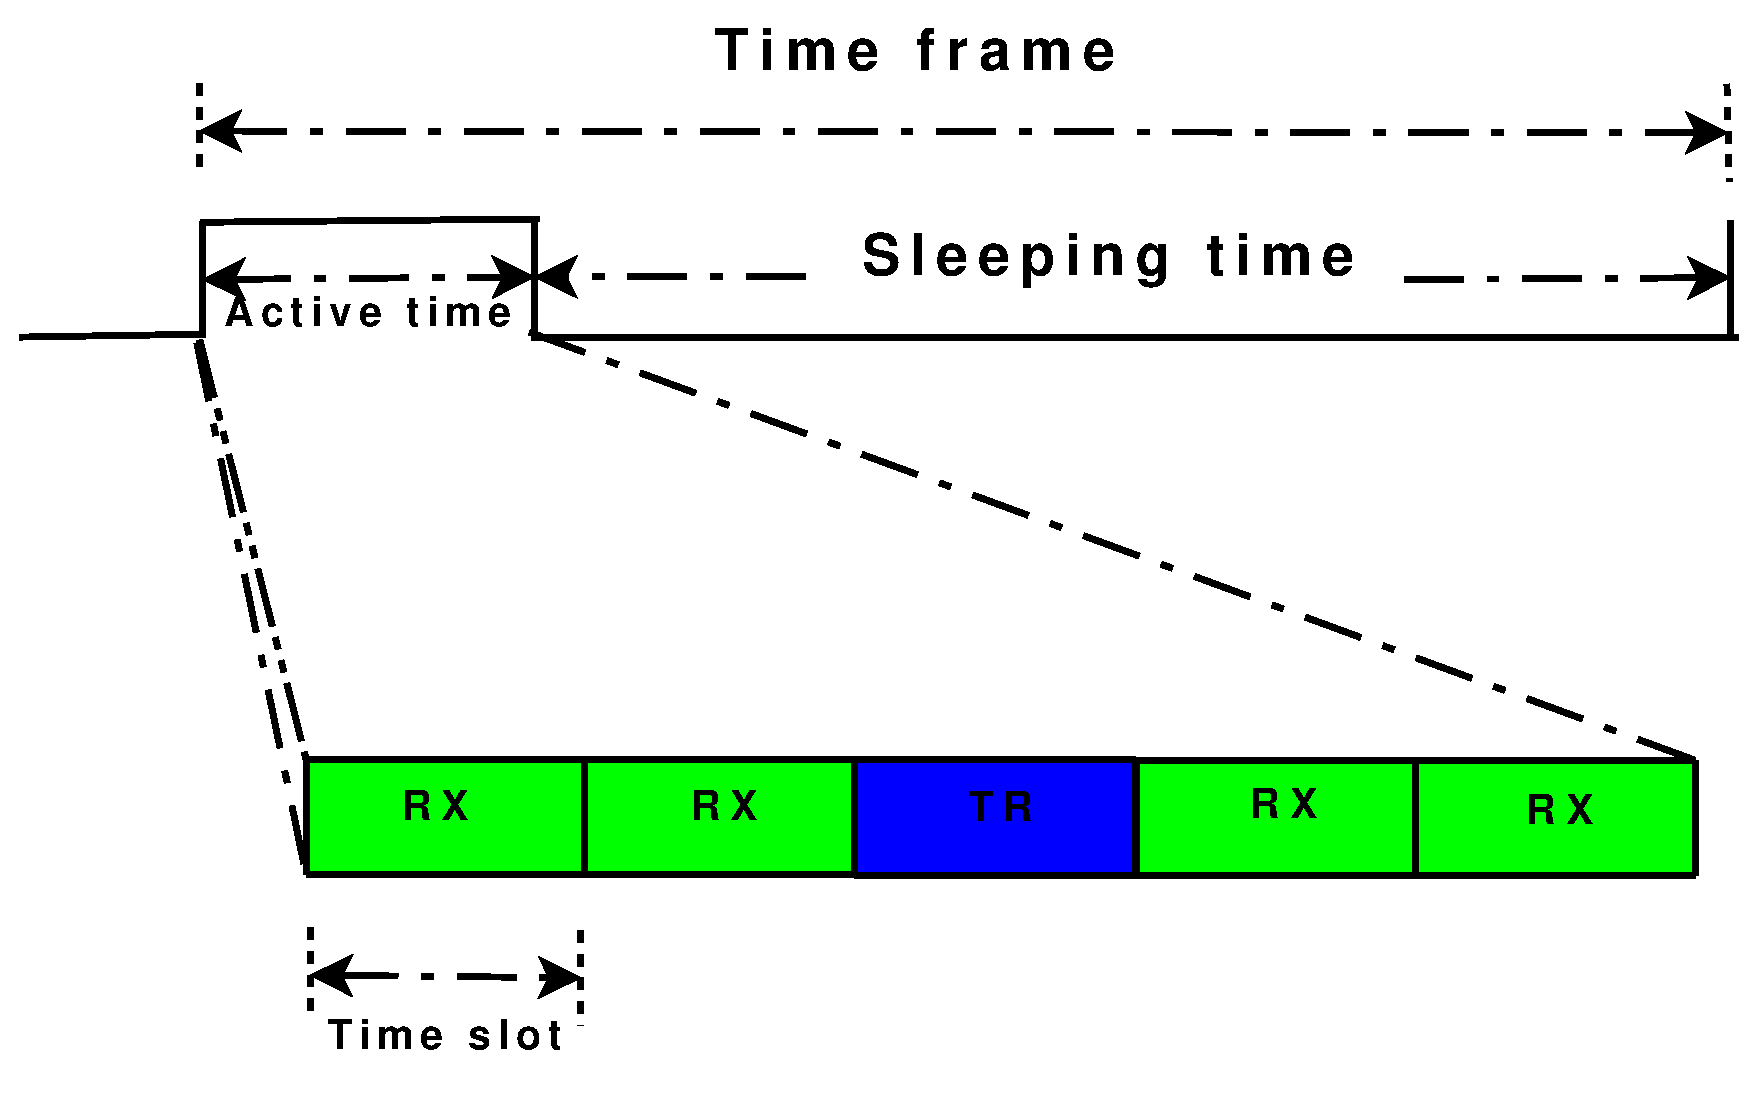
\includegraphics[width= 0.5 \textwidth]{tdmaframe}
\caption{TDMA frame}
\end{figure}
Thus, the master schedule, $T_o$ moment is adopted by the slave
node. Hence, if a slave has a TDMA schedule that is not in sync with
the master schedule, it re-synchronize on the received values. This
situation is very likely to happen in the network setup phase.
Rarely, when a node drifts due to the environment influences
(temperature, humidity). Once a slave node is aware of the master TX
slot, it locks the current RX slot, asserting the $n+1$ variable of
the slot as the current slot is free of collisions. Then, it chooses
its own transmission slot out of the remaining active slots that are
not locked. Here, we can see that a node needs $n$ active slots for
a collision less communication, where H is the number of neighbors.
The extra slot is used for the local transmission round. However,
this number is limited by the power and network data rate
requirements. A slot assigned as TX may change back to RX with a
probability $P_o$. This probability is computed at compile time in
function of the dynamics of the environment. This action is taken to
avoid possible collisions. In G-MAC is one such Node-schedule based
TDMA protocol. In this, time is divided into a number of different
slots as shown in Figure 4. The number of visible slots, five, have
been picked arbitrarily in the figure and do not map to the
selection in the simulation. Also note that the idle slots are not
being shown. The number of slots is fixed, ensuring that the
duty-cycle can be predicted perfectly. One consecutive set of
receiving slots, transmission slot, and idle slots make up a frame.
The nodes all run their own schedule. There are one or more
receiving slots, this is where data streams into the node. And there
is only one transmission slot. This is where data streams out of the
specific node. One such transmission slot consists of a certain
guard time at the beginning and at the end of the slot. This to make
certain that the drift is accounted for. The G in G-MAC comes from
Gossiping.
\begin{figure}
\centering
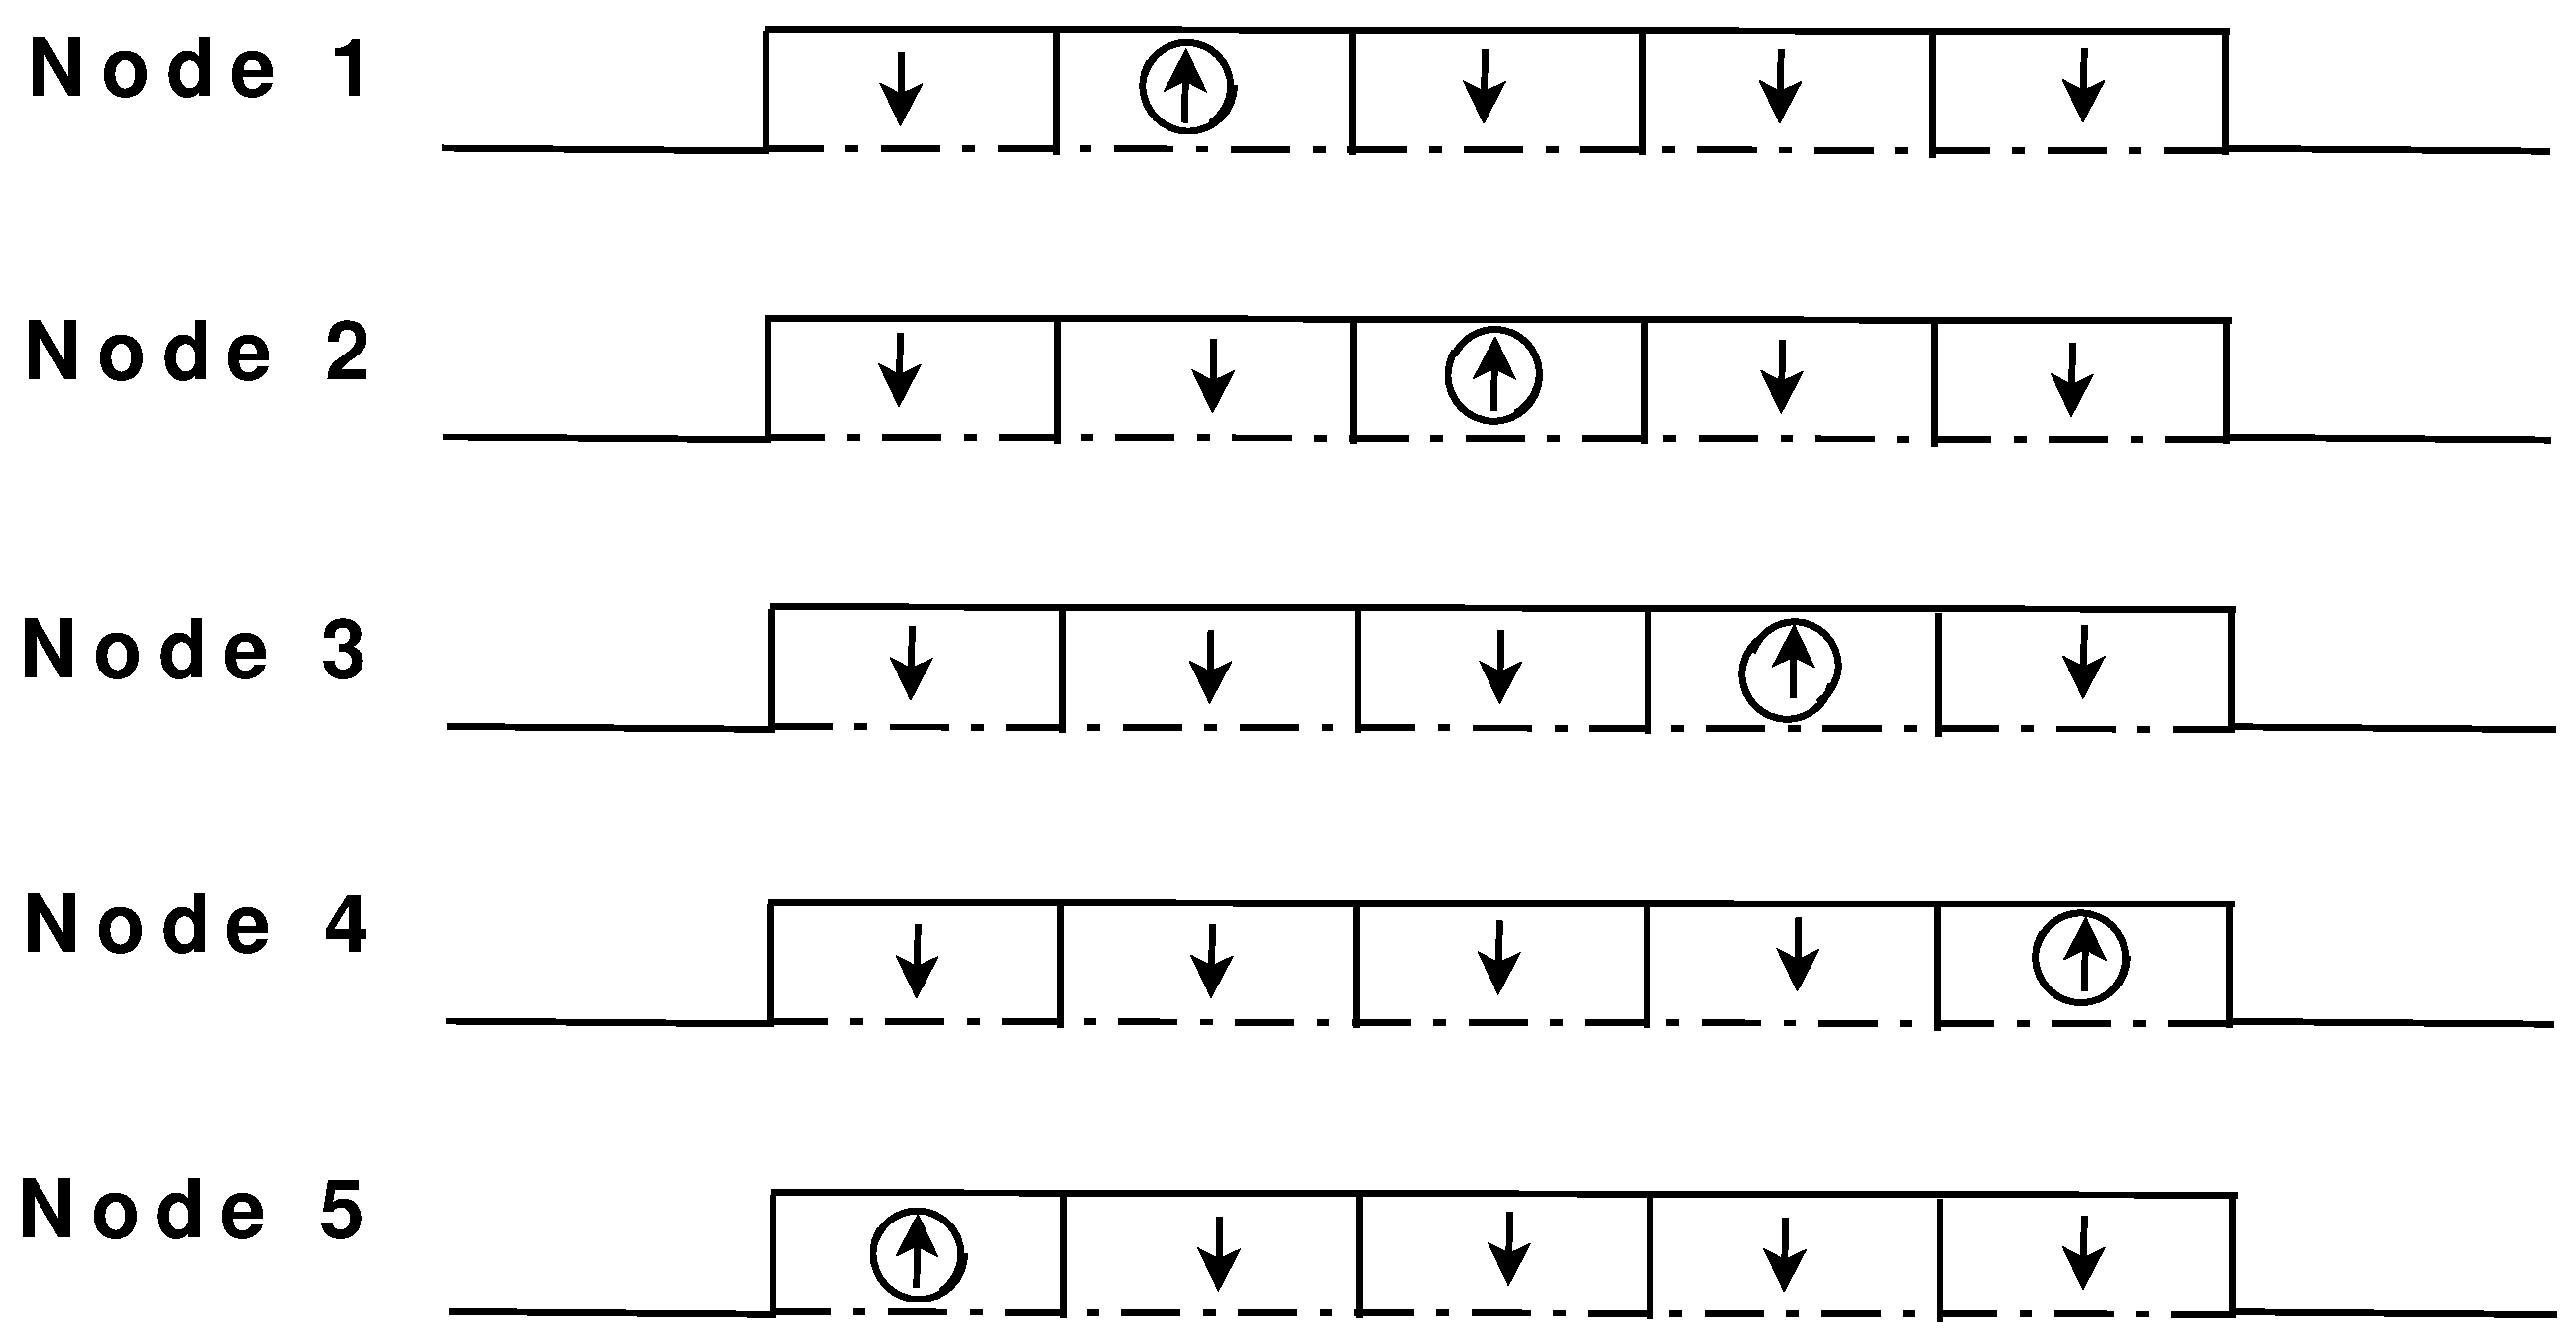
\includegraphics[width = 0.5 \textwidth]{tdmaschedule}
\caption{TDMA slot assignment}
\end{figure}
In order to have a seamless communication between the nodes, the
synchronization of the frames is a necessary part of the Mac
protocol. A sensor node has some drift in the timing frequency due
to physical factors. This causes the nodes to run out of sync. Given
that there is a certain error, the node will adjust its wakeup time
at the end of the last RX slot with the offset calculated with an
algorithm. As mentioned before, networks can drift out of sync with
each-other, forming multiple subnets. To reconstruct these into one,
nodes send out a re-synchronization packet in a random IDLE slot. If
this falls inside an active slot from the other subnet (say B) its
RX slot, that will finish its sending cycle and reschedule for a
wakeup at the starting point in time of subnet A. The case when we
have more neighbors than receiving slots, the TX slot will not
change as all the RX slots are locked. We assume that we know at
compile time the maximum connectivity of a network. Hence, the
number of active slots is chosen accordingly. A RX slot is unlocked
when the node does not receive any message for a period longer than
the synchronization period $T_{sych}$. The synchronization period is
a maximum time duration that is required to clock synchronize two
nodes. The effects of this time constant are discussed in the next
subsection. When a node changes its position in the network the
local schedule loses coherency with the neighboring nodes. Thus we
have to recompute the position of the TX slot accordingly to the new
neighbor schedules.
\subsection{Time Division Multiple Access}
The multihop communication can reduce the power requirements for a
node. Theoretically, as the attenuation increases at least
quadratically with the distance, it is more beneficial from
power-consumption viewpoint to use two hops of length $L$ than a
single hop of length $2L$ Another way to deal with power leakage of
the radio subsystem is to use duty cycles. A duty cycle is fixed
length of time which is divided into a communication time and
sleeping time. We can have major benefits by using this scheduled
communication/sleeping protocol:
\begin{itemize}
 \item low duty cycles - a node can operate in low duty cycles;
\item efficiency in transmission - a sender can efficiently transmit a message to its
neighbor by just waking up and sending exactly when a receiver is
listening.
 \item efficiency in receiving - a receiver can schedule
its own time intervals to receive a particular neighboring
transmitter. \end{itemize} We assume that in a communication round,
all the nodes that are in each other range communicate only once
their cache using broadcast. Theoretically, a node that broadcasts
sends the entire content of its cache to all its neighbors. However,
in real life we send only a fraction of this cache, usually only an
entry, message of the local cache. An other assumption is the
exchanging of the cache during one communication round. Thus, the
communication initiator as well as the receiver have the entire
content of each other cache. However, in the proposed implementation
we do not assume this behavior as a communication pattern. The
environment may be polluted with noise and the message exchange is
damaged, resulting in corrupted messages at the receiver. The
success of the communication is related to the probability that a
noise to interfere with the broadcast communication. As high is the
noise probability, as low is the communication probability. The safe
belt of this protocol is represented by the presence of the gossip
cache. This cache holds messages that are not necessarily useful for
the current node. Thus, achieving a communication redundancy. So,
although a message failed to reach all its destinations, it may
reach the destination in one of the next communication rounds. In
this protocol we do not need to implement an ACK/NACK communication
scheme to ensure that a message has been received in good
conditions. The communication quality of service is guaranteed by
the gossiping layer probabilistic features. The scheduled
communication/sleeping protocol, the multihop scheme and the
rippling of the message through the network are best implemented
using a time division multiple access (TDMA) scheme. A TDMA based
protocol divides time into time slots, which nodes can use to
transfer data without reserving the medium or collisions. Usually,
this medium access scheme is best suited for the infrastructure mode
where the base stations schedule the TDMA slots for each sensor
(e.g. GSM). However, in our network we do not make use of such
structure, the scheduling of the TDMA slots is made locally by
reaching an agreement between direct neighbors. The proposed
protocol is not guaranteed $\%$collision free. Whenever a collision
is detected by a node, it changes the local variables trying to
solve this issue for the next transmission time.at we need two kind
of synchronization: the TDMA schedule synchronization and the clock
synchronization. While the TDMA schedule synchronization is
susceptible to be called only once at the network setup moment, the
clock synchronization is requested each time a node receives a
message, keeping an internal oscillator to not drift from the given
$T_o$ moment.Each node has a crystal oscillator that has a certain
accuracy, which results in time drifts. This causes the TDMA time
slot boundaries to drift when we compare two nodes with the same
schedule. There are several factors that affects the clock accuracy,
like temperature. The clock drift rate is a fundamental physical
limit. To accommodate potential clock drift, the listening time
within a RX slot is extended with a guard time, Figure
$\ref{fig:guardtime}$.
\chapter{Problem Formulation}
\section{Clock and Frequency standards}
The quality of a clock usually boils down to its frequency stability
that is, the ability of its frequency standard to emit events at a
constant frequency over time. The absolute value of the frequency
compared to the desired value or, its frequency accuracy|is also
important, but calibration can easily compensate for an inaccurate
but stable standard.
\newline The focus of our work is on methods of clock synchronization,
not on construction of better clocks. However, clocks are very
important: the error bound achieved by a clock synchronization
method is linked to both the error inherent in the method itself,
and the stability of the clocks' frequency standards. In fact, to
some extent, the two are interchangeable. Stable clocks can
compensate for a synchronization channel between them that is prone
to large (but unbiased) errors: many synchronization events can be
averaged over a long time. Similarly, a precise synchronization
channel can compensate for a poor-stability frequency standard;
frequent synchronization minimizes the time in-between when the
clock is left to fend for itself.
\newline
Many types of frequency standards exist. In general, as their
stability and accuracy increase, so do their power requirements,
size, and cost, all of which are important in sensor networks. Most
commonly found in computer clocks are quartz crystal oscillators,
characterized by $\cite{19}$. Quartz crystals are attractive because
they are inexpensive, small, use little power, and perform
surprisingly well despite their low resource requirements. The
frequency generated by a quartz oscillator is affected by a number
of environmental factors: the voltage applied to it, the ambient
temperature, acceleration in space (e.g., shock or attitude
changes), magnetic fields, and so forth. More subtle effects as the
oscillator ages also cause longer-term frequency changes. The
inexpensive oscillators commonly found in computers have a nominal
frequency accuracy on the order of between $10^4$ to $10^6$ that is,
two similar but uncalibrated oscillators will drift apart between 1
and 100 microseconds every second, or, between about 0.1 and 10
seconds per day $\cite{19}$. However, their frequency stability is
significantly better with a change in frequency of one part in
$10^9$ to $10^11$ when averaged over several seconds or more.
\newpage
\section{Sources of synchronization error}
The first step in designing any time-synchronization algorithm would be to under-
stand why and where it is required. The different factors which give
rise to errors in clocks of nodes or in synchronization algorithm
can be divided into two main categories:
\begin{enumerate}
\item Oscillator Characteristics: The sensor nodes clocks run on very cheap oscillators.
      The following two characteristics are the main sources of errors between the clocks
      of two different nodes.
      \begin{itemize}
         \item Accuracy: This is a measure of difference between oscillators expected (ideal)
           frequency and actual frequency. It is also called as resolution of the clock; its
           maximum is specified by the manufacturer.
         \item Stability: This is oscillator tendency to stay at the same frequency over
           time. There can be short-term instability due to environmental effects, supply
           voltage etc.; or long-term instability due to temperature effects, oscillator
           aging etc.
      \end{itemize}
\item System and Network issues: The non-determinism in the message delivery latency
      is a major source of error in any synchronization algorithm, when applied into real
      sensor networks. This can be categorized in four type of
      delays:
      \begin{itemize}
         \item Send Time: The time spent at the Sender of the times tamps to build the
          message, i.e. the time duration between generating the times tamp and injecting
            it into the network.
         \item Access Time: Delay occurred while waiting for access to the transmit channel.
         \item Propagation Time: Time required for the message to travel from sender to receiver.
         \item Receive Time: Time needed for processing at the receivers network interface.
      \end{itemize}
\end{enumerate}
      All the above factors result in following errors between the clocks of two nodes:
\begin{itemize}
\item Phase error: The oscillators of any two nodes can be out of phase at
any given time, resulting into different time on both clocks. There
can be some initial time-offset between nodes at the start of a
synchronization procedure.Phase error is an instantaneous metric: at a given moment, how far apart are
these clocks?
\item Frequency error: Frequency error, in contrast, measures the difference in the clocks’
rates. This metric is important because it predicts the growth of phase error over
time. That is, if clocks are perfectly synchronized now, at what rate are they
drifting apart? How well will they be synchronized in 60 seconds?
\item Clock drift: It is not just that the clocks are running at different rates, but even
the frequency of each clock does not stay constant over a period of
time! Clock drift arises from the instability of oscillators,
because clocks drift from their initial frequency. For instance, if each clock
drifts at a rate of R msec/sec, then maximum relative drift between
two clocks can be 2R msec/sec.
\end{itemize}
      Even if two clocks are assumed to have the same frequency and no drift, the above
mentioned delays in the network result in phase offset between two
clocks. This is because when the timestamp from the sender reaches a
receiver, the receiver adjusts its clock according to the received
timestamp; but the sender's clock changes in the time required for
the timestamp to reach the receiver, due to network delays.
      For a network of nodes, these sources give rise to errors in accuracy from an ideal
clocks, and dispersion amongst their clocks.
\section{Clock Drift and Delay}
\subsubsection{Drift} We will now present an expression for the clock
drift or phase error between two clocks. If we subtract the current
time in one clock from the current time in other clock, we get the
time-offset or error between them, at the current point of time. So
predicting the value of this time-offset will be same as predicting
the time in the clock of other node.
      From the definition of frequency:
\begin{equation}
f = d\phi/dt \label{freq_defn}
\end{equation}
and integrating both sides over time,
 \begin{equation}
\phi =\int f(t)dt
 \end{equation}
where
      f = frequency
      $\phi$ = phase
      t = time\newline
     \newline The clock time is described as
\begin{equation}
C(t) = k\int_{t_o}^{t} {\omega(\tau)d\tau} + C(t_o) ,
\end{equation}
where $w(\tau)$ is the frequency of the clock and k is the constant.
The exact clock drift is hard to predict because it depends on
environmental influences (e.g., temperature, pressure, power
voltage). One can usually only assume that the clock drift of a
computer clock doesn't exceed a maximum value $\rho$ . This means
that we assume:
\begin{equation}
1-\rho \leq \frac{dC(t)}{dt} \leq 1+\rho
\end{equation}
where $\rho$ represents the maximum clock skew.A typical value for
$\rho$ achievable with today's hardware is $1e-6$ which means that
the computer clock drifts away from real time by no more than one
second in ten days, which is still a significant value. Note that
different computer clocks have different maximum clock drift values
$\rho_i$.\newline The frequency of the clock is dependent on many
factors and is given as
\begin{equation}
\omega_i(t) =f(\omega_o, \Delta
\omega,\omega_d(T-T_o),\omega_e\Delta t,\omega_r) \label{frequency}
\end{equation}
where\newline
      $t_0$ = starting time \newline
      $\Delta_t$ = the age of the oscillator , working time  \newline
      $\omega_o$ = nominal frequency \newline
      $\omega_e$ = frequency error due to ageing effect \newline
      $\Delta \omega$ = calibration error \newline
      $\omega_d$ = frequency error which occurs due to temperature \newline
      $\omega_r$ = short-term frequency instability (noise) term \newline
The above equation provides a good approximation for all common
oscillators. The nominal frequency can also be identified as the
ideal frequency at which the oscillator is supposed to run.
Combining the equations $\ref{frequency}$ and integrating from the
starting time $t_o$ to the current time t, we get,
\begin{equation}
t_i(t) - t_i(t_o) = \frac{1}{\omega_o} \int^{t_o}_{t}\omega_i(t)dt
\end{equation}
The short term frequency variation has zero mean and does not lead
to accumulated time errors. Also the amplitude of these short term
variations (clock jitter) is small enough that they do not cause the
clock to accelerate or decelerate in a very large amount. But the
environmental term, primarily due to temperature, can be
significant. From the about equation, we have derived the expression
for clock drift or time offset between clocks of two nodes - a
sender and a receiver. Assume that these two nodes clocks are of the
same type and therefore, under ideal conditions, they should run at
the same frequency, say $\omega_o$ , without any initial phase
error. But this is not possible in reality, and so each of the
clocks will drift from its ideal conditions.
     Thus, the phase or time offset between two clocks at any given time results from a
combination of initial phase offset, frequency bias, calibration error, frequency drift
and the environmental terms. As more time passes from the
synchronization point, the drift and environmental terms become more
significant.
       This resulting expression is used as a model for designing the solutions, as well as
for data simulations.
\begin{figure}[b]
\centering 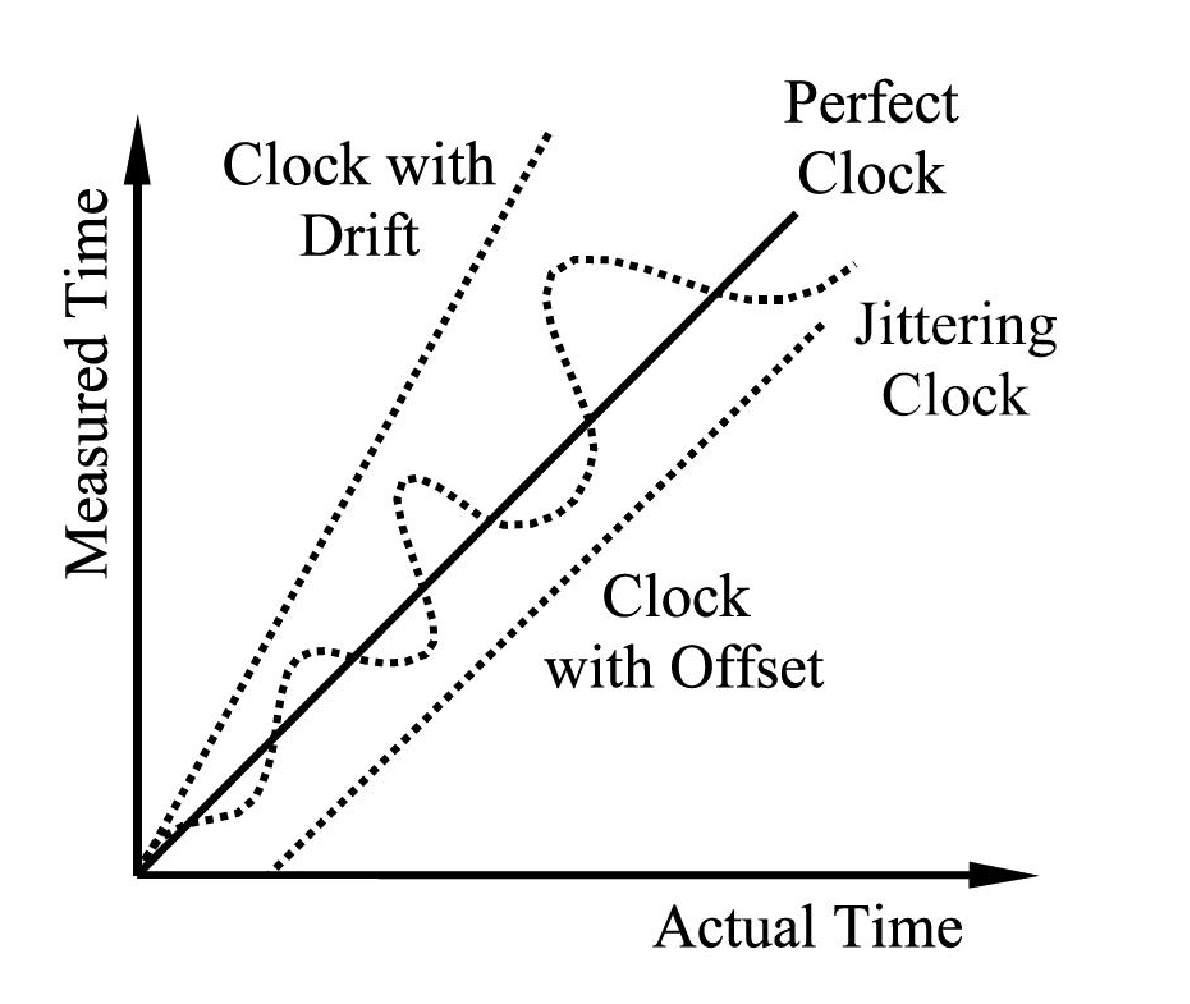
\includegraphics[width=0.5
\textwidth]{actualvsmeasuredtime} \caption{Measured time versus real
time} \label{fig:clocktimevsrealtime}
\end{figure}
\subsubsection{Message Delay} The other source of error which arises
between the sensor nodes is due to the dealy in the transfer of
messages between the sender and the reciver node. This is inculed in
the system and networks category of the errors that the clock
doesn't have any effect on it. This delay is comprised of the
following:
\begin{itemize}
         \item Send Time: The time spent at the Sender of the times tamps to build the
          message, i.e. the time duration between generating the times tamp and injecting
            it into the network.
         \item Access Time: Delay occurred while waiting for access to the transmit channel.
         \item Propagation Time: Time required for the message to travel from sender to
            receiver.
         \item Receive Time: Time needed for processing at the receivers network interface.
\end{itemize}
Send Time : It is the time it takes compose a message and send it to
the channel. It is calculated to be $1e-6$. \newline Access Time:
Time it takes to access the channel. It is estimated to be $1e-6$.
\newline Propagation Time: Time it takes for a message to reach the
receiver location. It is again estimated to be $1e-6$. Receive Time:
Time it takes to process the received message. It is estimated to be
$1e-6$.
\section{Requirements of the Algorithm}
\subsection{Lifetime}
Lifetime is the interval that clocks remain synchronized, or the
interval over which a particular timescale is defined. Sensor
networks need synchronization over a wide range of lifetimes,
ranging from less than a second to timescales that are
persistent.\newline In our implementation here, the length of
lifetime required is throughout the life time of the network since
the primary reason for the synchronization is for TDMA frame
synchronization. Thus, a proper synchronization is required for a
seamless communication to happen between the nodes.
\subsection{Scope}
The scope is the size of the region in which a timescale is defined.
In some cases, the scope may be purely geographic (e.g., distance in
meters). In other contexts, it is more useful to think about the
logical distance, such as the number of hops through a network.
Naturally, these two forms are correlated in a sensor network,
scaled by its radios nominal range.\newline In this thesis,
exploration of a global synchronization algorithm is conducted.
Hence, a node moving across the field, should be synchronized to the
remaining nodes, which it might join again after some periods. A
disruption of communication can also result in the disappearance of
a node where after some periods of out-of-sight, a communication
link can be established again. During the 'comeback', the node
should be able to adapt its clock to the remaining nodes in the
neighborhood.
\subsection{Internal vs. External}
In many distributed systems, network time synchronization simply
means adjusting the clock to a correct time from an outsider. This
definition implies that a notion of the correct time exists.
Typically, the time is UTC the international standard for civil
time. However, in sensor networks, UTC not always needed. Indeed, in
some cases, the definition of an SI second itself may not be
relevant. In other words, there are situations where distributed
nodes need to be synchronized, but not necessarily running at a
particular frequency known a priori. As an example, coordinated
actuation is needed in some applications which need to plan for
collaborative action. In many cases, the exact time at which the
plan is executed is far less important than ensuring that all nodes
act simultaneously. This includes TDMA frame scheduling. This
application requires internal or relative synchronization: the
network must be internally consistent, but its relationship to
outside time standards is not needed or known. So, in this thesis,
internal synchronization is explored.
\subsection{Energy Budget}
The need for energy efficiency pervades virtually all aspects of
sensor networks design. The exact energy constraints are difficult
to quantify because there is a wide range of hardware found across
the spectrum of network implementations, and often within a single
network. Some nodes have large batteries and run all the time;
others are so constrained that they only wake up occasionally, take
a single sensor reading, and transmit it before immediately
returning to sleep.\newline The sensor nodes that we are going to
implement the synchronization algorithms run by ... batteries.
Energy budget is a big constraint in the quest for the new algorithm
for the synchronization of the nodes. A trade-off between the
performance of the algorithm and the increase in energy consumption
can be taken as a bait.
\subsection{Convergence Time}
The importance of convergence time as a metric is directly tied to
the need for energy efficiency. If energy were not a concern, our
chosen form of synchronization could simply be left running
continuously. Though convergence time might be important due to its
effect on network startup, it would make no difference in the
steady-state. However, in this energy-constrained world, systems are
often forced to power down as many services as possible for as long
as possible. This makes convergence time important to
consider.\newline Convergence is expected to be at 9 clock cycles,
the difference between the maximum and the minimum should be in the
range of the guard time so that the message received falls in the
receiving slot of the receiver frame.
\subsection{Simplicity}
An overhead in the message is avoided. A time stamp is not needed in
the frame in order to decrease the message overload. Thus, there is
no additional information passed on the frame which can be used in
the synchronization of the nodes. This inturn has an advantage in
the energy constraint WSN. Although it passes most of the burden to
the algorithm to determine the next wakeup time of the node.
\newpage
\chapter{Synchronity protocol}
\section{Synchronization Frequency}
In achieving the clock synchronization for a frame synchronization
in a TDMA scheduling, a guard time is given for a fault tolerance
which is used to accommodate the phase errors. In its downturn, it
consumes energy as the guard time increases.\newline Decreasing the
timing of the synchronization and do periodic execution of the
synchronization of the algorithm greatly reduces the energy
consumption of the wireless sensor network. Thus, a synchronization
frequency is defined as the period in which the network can stay
synchronized without being synchronized.
\begin{figure}
\centering
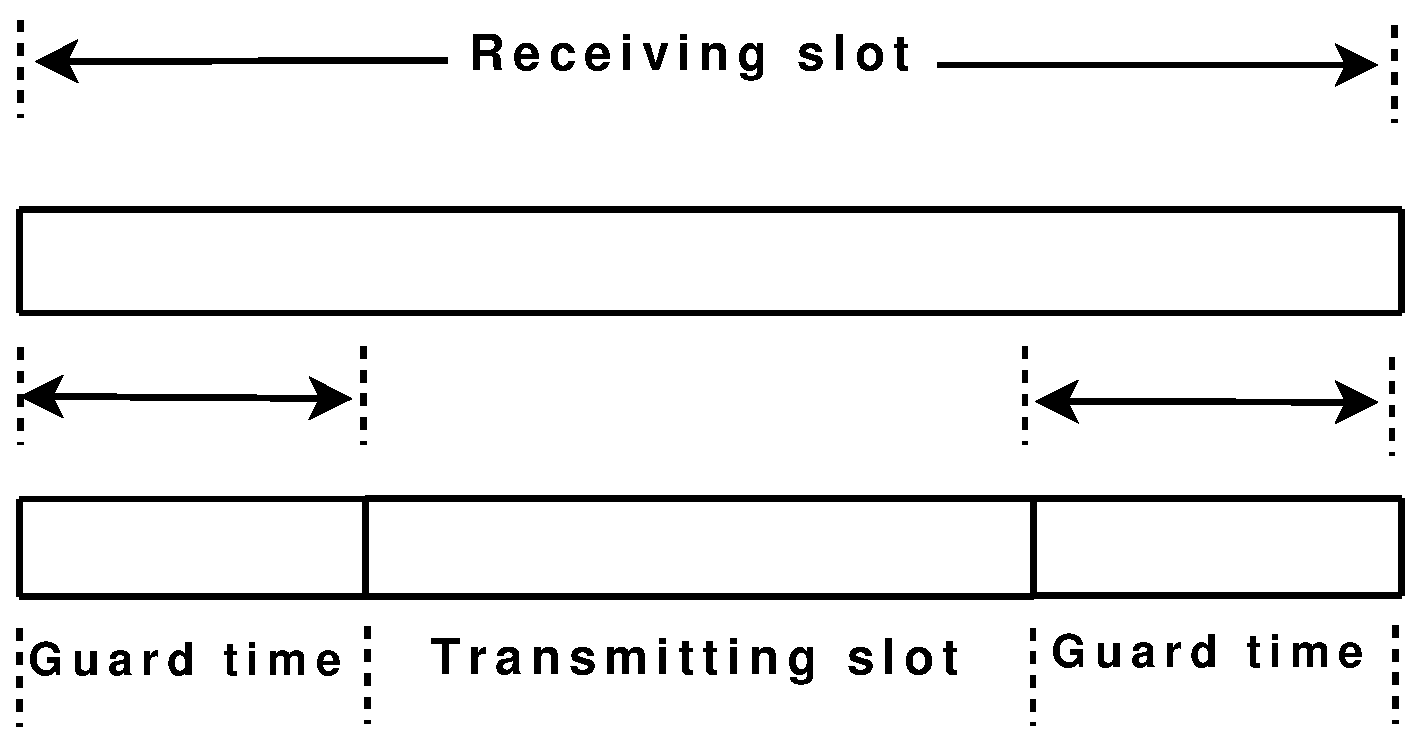
\includegraphics[width = 1 \textwidth]{guardtime}
\caption{Guard time of the nodes}
\label{guardtime}
\end{figure}
\newline We can define a time slot as being expressed in a
number of clock cycles $k_o$ as
\begin{equation}
t_{slot} = \frac{k}{\omega_o} ,
\end{equation} where $\omega_o$ is the frequency of the clock and
$t_{slot}$ is the duration of a slot(transmitting or
receiving).\newline If  we consider that we have a synchronization
period $T_{synch}$ and the maximum clock drift of a clock $\theta$ ,
then the maximum time difference between a sender and a receiver is
\begin{equation}
t_{diff} = 2T_{synch}\theta
\end{equation} where the factor of
two reflects the worst case scenario where each node's clock drifts
in the opposite direction.\newline Since the relative time
difference between two nodes can be in two direction, the guard time
needs to be twice $t_{diff}$. Thus,
\begin{equation}
t_{guard}= 2t_{diff} = 4T_{synch}\theta.
\end{equation}
At this end, we can write the minumum duration for a time slot
$t_{slot}$ as being
\begin{equation}
t_{slot} \geq t_{guard} + T_{tx},
\end{equation}
where $T_{tx}$ is a system constant and it represents the required
time to send a packet from one node to other. Comparing the
equations above,
\begin{equation}
k_of_{xtotal} \geq t_{guard} + T_{tx}.
\end{equation}
Thus, each message that is send within a time slot is exactly
received by a neighbor at a known clock tick number
\begin{equation}
tick_{rx} = [\frac{T_{tx}+\frac{t_{guard}}{2}}{f_{xtotal}}]
\end{equation}
Hence, each time when a node receives a message, it has to be
received exactly at the clock tick given by equation 10. Whenever
this number is not equal with the desired one, we set the slot tick
counter to $tick_{tx}$. This easy mechanism adjusts the clock drifts
at the receiver side. The resolution is given by the clock frequency
and comply to the following proposition: as fast the clock is as
high the resolution is. A general rule to chose $f_{xtotal}$ is
\begin{equation}
\frac{t_{guard}}{4f_{xtotal}} \geq 1.
\end{equation}
Two nodes have a good communication link if they synchronize their
clocks at least once every $T_{synch}$ fact that give us the
following relation
\begin{equation}
T_{synch} \geq (n+1)t_{slot} + C_ot_{slot},
\end{equation}
where $C_o$is a system constant, derived from the desired
communication duty cycle.\newline It is a good practice to desig
systems having a $T_{synch}$ greater than the time frame. This
improves the noise tolerance of the system, however, on the other
hand, it decreases the lifetime of a node. To obtain the value of
$T_{synch}$ for a particular system with a given duty cycle we have
to solve the next problem
\begin{equation}
t_{guard} \geq 4\theta T_{synch}
\end{equation}
\begin{equation}
t_{slot} \geq t_{guard} + T_{tx}
\end{equation}
\begin{equation}
T_{synch} \geq (n+1)t_{slot} + C_ot_{slot}
\end{equation}
There is a trade-off in determining $T_{synch}$: increasing
$T_{synch}$ by changing the value of $C_o$ reduces the energy costs
of sending messages, on the other hand we increase the cost of guard
time and decrease the network performance (data rate), see Figure .
A smaller amount of messages per minute means a longer $T_{synch}$.
\newline From the datasheet of the crystal clock $\cite{1}$,
the frequency of the clock is affected by different factors.
\begin{equation}
\omega_i(t) = f(\omega_o,\Delta \omega ,\omega_d(T-T_o),\omega_e,
\omega_r(t))
\end{equation}
where \newline $\omega_o$ is the nominal frequency \newline $\Delta
\omega$ is the calibration error \newline $\omega_d$ is the
frequency error due to temperature \newline $\omega_e$ is the ageing
effect \newline $\omega_r(t)$ is the random noise effect ,
distributed normally across time \newline Assuming the maximum
deviations and using the data presented in $datasheet$, we can get
the maximum deviation to be
\begin{equation}
\theta = 30 ppm
\end{equation}
This is the minimum size of the guard time that should be in order
to accommodate the clock drift. Thus, the wakeup time difference
between the nodes in the synchronization algorithm should at the
minimum be at this threshold guard time.
\newline
Parts per million is the factor in which a measurment of the clock drift where
the drift is measured in microseconds.
\newpage
As it is described earlier, the firing time of the nodes should be
synchronized to an extent in such away that the nodes are
synchronized in the long term. The difference in the transmitting
times of the nodes is
\begin{equation}
\Delta t_{ij}^{(n)} = t_i^{(n)} - t_j^{(n)} ,
\end{equation}
where $t_i$ and $t_j$ are the wakeup times of Nodes i and j at the
$nth$ period. The transmitting time of a node at a random time after
t after it is turned on is
\begin{equation}
t_i^{(n)} =  f_it + t_{io},
\end{equation}
where  $f_i$ is the frequency of the crystal clock and $t_{io}$ is
the initial startup time of the node. The frequency of the node
varies due to the different factors mentioned above.
\begin{figure}
\centering
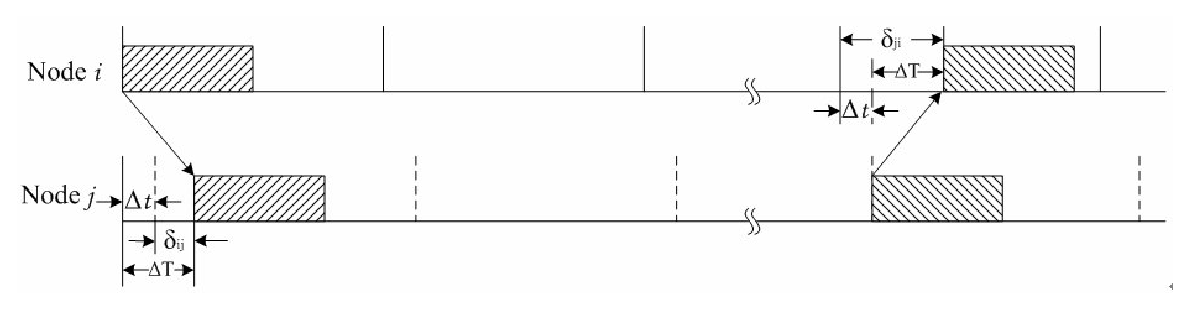
\includegraphics[width=0.8\textwidth]{node_time}
\label{node_time}
\caption{How the node time is different}
\end{figure}
Thus, the difference in the wakeup time of the nodes is given by
\begin{equation}
\Delta t_{ij} = f_it + t_i{ o}- (f_jt + t_{jo} ),
\end{equation}
\begin{equation}
\Delta t_{ij} = (f_i - f_j)t + (t_{io}-t_{jo}),
\end{equation}
Since the frequency distribution of the nodes is normally
distributed, the difference in the frequencies is also normally
distributed. So, in the long run, the time difference between the
nodes is increasing [$\ref{fig:clocktimevsrealtime}$]. Thus, the
offset being applied should be able to compensate for the phase
error introduced by the drift as well as the frequency changes. Two
ways to accomplish this. The first one is adjusting the clock
frequency to come up with a better transmitting time. The second one
is to adjust the next transmitting time depending on the current
transmitting times of the node and its neighbors. In this thesis, we
will explore the second option due to the reasons stated below.
\begin{itemize}
\item The cost of adjusting the frequency of the clock is by far more
expensive than adjusting the next transmitting time of the node.
\item The complexity of the implementation is larger which in turn
results in more energy consumption.
\end{itemize}
Application of offset compensating. Thus, the next transmitting time
of the node is dependent on the current transmitting time of its
neighbors in relation to its current transmitting time. We will
denote the next transmitting time as $\tilde{t}$. Thus,
\begin{equation}
\tilde{t_i} = t_i + SLOTTIME + \xi_i ,
\end{equation}
where $SLOTTIME$ is the time duration of a slot and $\xi_i$ is
given by
\begin{equation}
\xi_i = f(\Delta t_{ij}) ,
\end{equation}
The function f is based on an algorithm which takes the transmitting
time differences between the node and its neighbors and determines
the optimal offset to be added to the transmitting time of the node.
\newline Different algorithms are presented here and discussed with the
simulation results presented in the last section of the projects.
\newpage
\section{Median algorithm and its drawback?} In this section, we
will see the median algorithm which is implemented and see the
results in the section.
\begin{itemize}
\item A transmitter broadcasts m reference packets.
\item Each of the n receivers records the time that the reference was observed,
according to its local clock.
\item Each receiver $i$ can compute its phase offset to
any other receiver j as the difference of the phase offsets implied
by nodes i and j. That is, given
\newline n: the number of receivers
\begin{equation}
\Delta t_{ij}^{(n)} = t_i^{(n)} - t_j^{(n)} ,
\end{equation}
\item The receiver computes the median of the received offsets
\begin{equation}
\xi_i^{(n)} = median(\Delta t_{ij}) ,
\end{equation}
\item The receiver adjusts its wakeup time by the computed offset
value.
\begin{equation}
t_{i}^{(n+1)} = t_i^{(n)} SLOTTIME - \xi_j ,
\end{equation}
\end{itemize}
\subsubsection{Gain factors}
As per the application of the median algorithms, there are drawbacks
on the implementation of the algorithms. In some test-cases, the
algorithms fails to converge or at least stays unsynchronized for a
certain period of time which might result in a disruption of
communication in the place where synchronization is essential.
\newline Here we present a typical scenario where interferancene of the cases where the median algorithm is .....Hence a
gain factor could be added to ensure a proper convergence of the
synchronization error. Different gain factors are applied and the
results are presented in the next chapter.
\begin{figure}
\centering
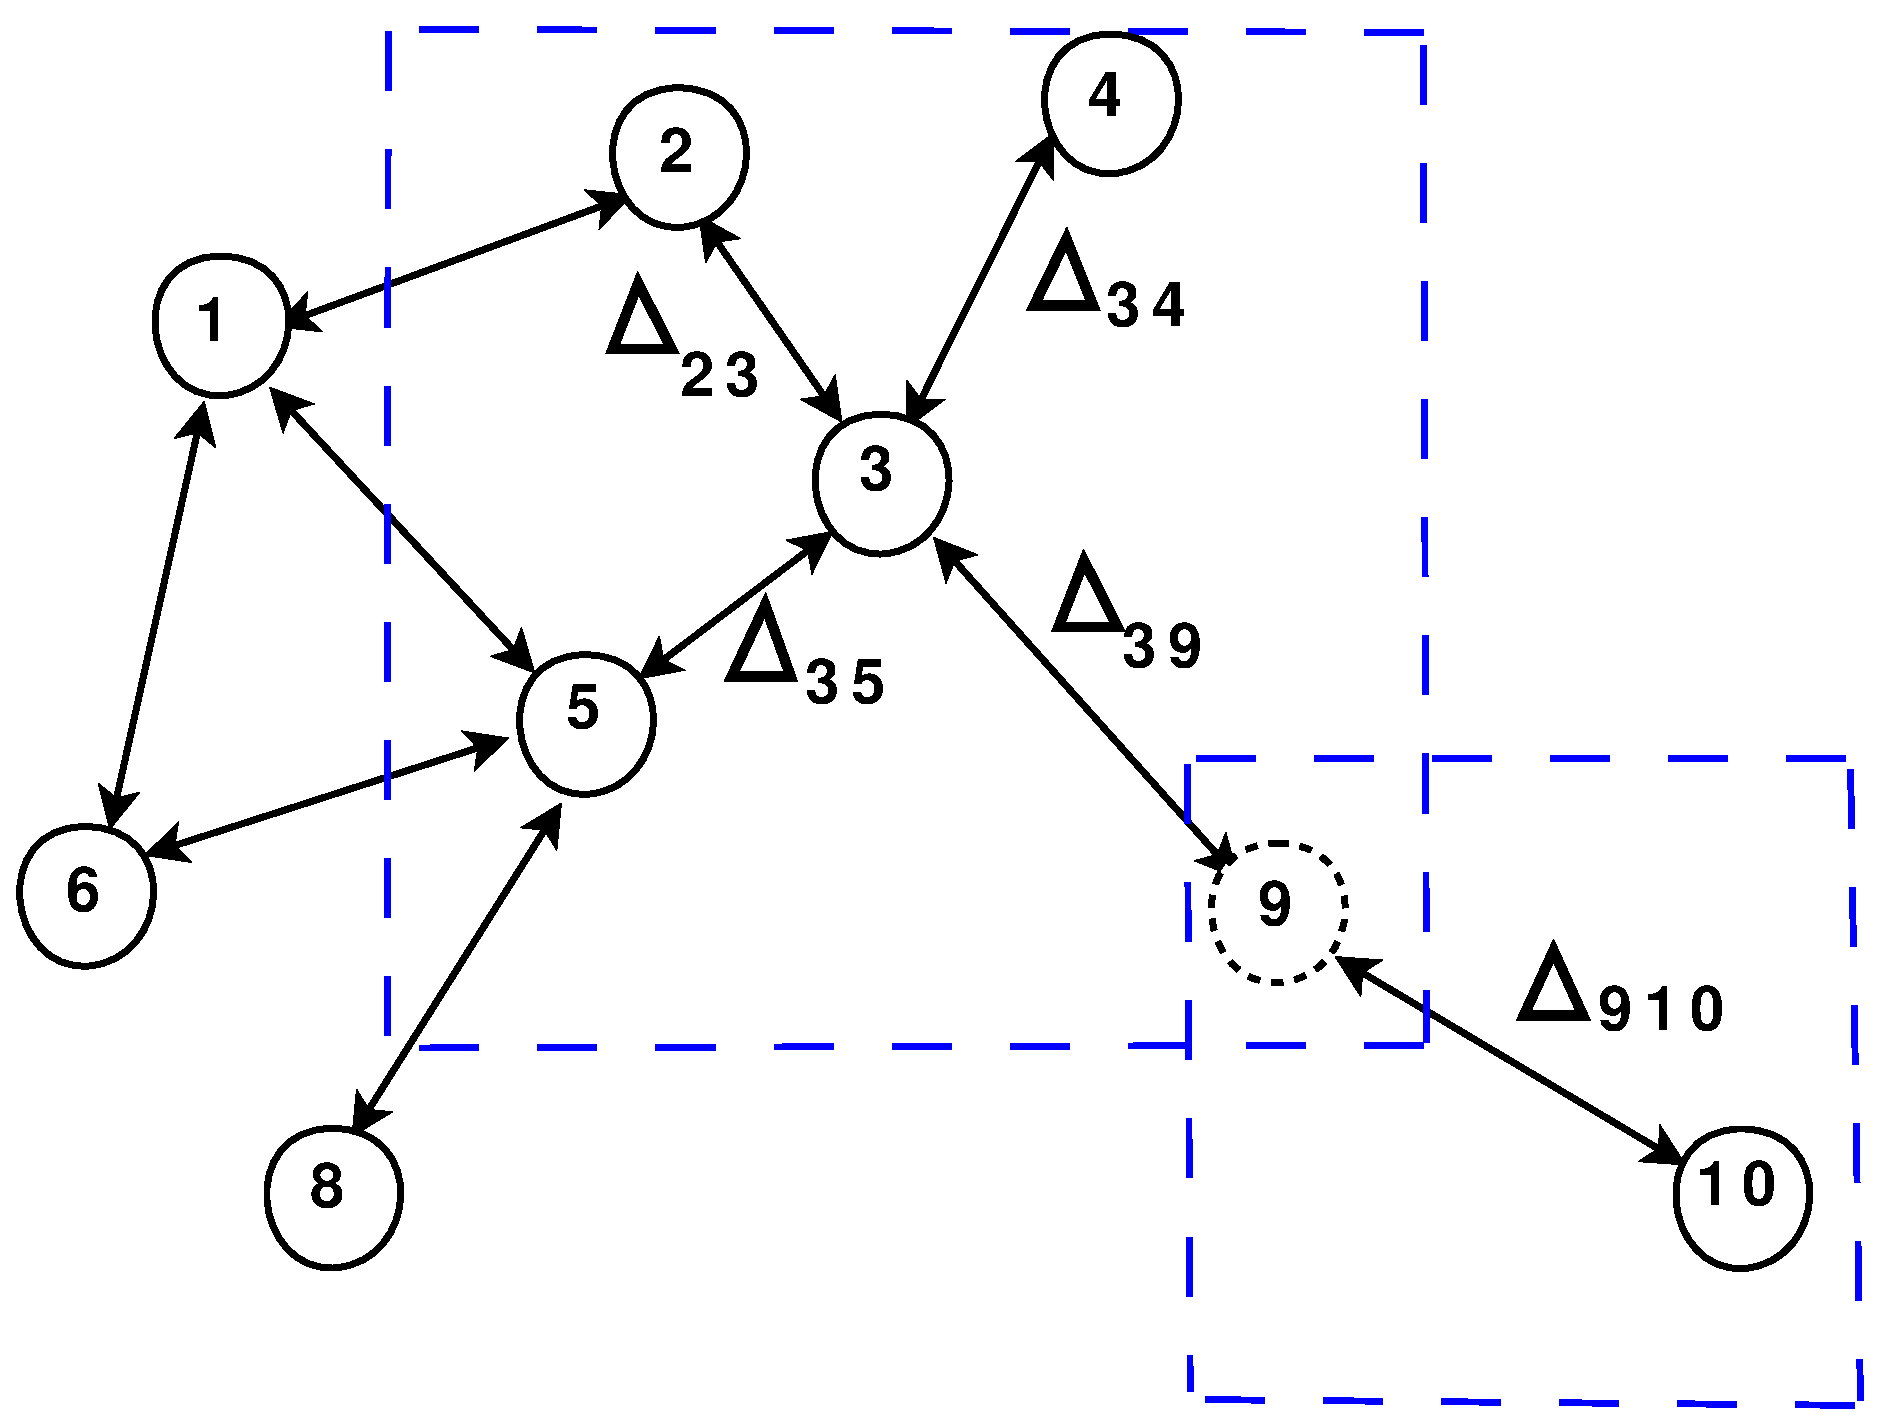
\includegraphics[width= 0.6 \textwidth]{node_field}
\caption{A WSN scenario}
\label{wsn}
\end{figure}
In the figure $\ref{wsn}$, Node 9 belongs to two broadcast domains.
Thus, upon the application of the median algorithm, the node tends
to adjust its wakeup time with the median of the offsets from its
neighbours, Node 3 and Node 10. Thus, adjusting the wakeup time,
\begin{equation}
\xi_9 = \frac{\Delta t_{910} + \Delta t_{39}}{2}.
\end{equation}
With node 10 being a new comer to the well established network, it
has , lets say , a major drift from the other nodes. Being in synch
with the other nodes, node 9 will drift away from the nework after
its adjustment with the node 10. Thus, it will take more time to
synchronize with the network again. Thus, the performance of the
median algorithm decreses with the dynamicity of the network.\newline
So, inorder to address this problem, a range of alogorithms are explored in the next sections
to realize an energy-efficient, stable and simple frame synchronization.
\newpage
\section{Weighted Measurments - Interferance-phobic}
One form of approach to tackle the appearance and disappearance of node, due to channel
conditions as well as collisions is a weighted-measurement approach.
Use cases or general expressions: A weight is added to the increase
the influence of the close by neighbors and ensure faster
synchronization. In addition to that, a new joining neighbor can get
synchronized with out disturbing the existing neighbors, adjusting
its time to the big swarm of nodes. Its a metaphor of "Majority
Wins".
\begin{equation}
\xi_i^{(n)} = \sum{w_{ij}^{(n)}\Delta t_{ij}^{(n)}} ,
\end{equation}
where $\sum{w_{ij}^{(n)}= 1}$. The next task will be how to choose
the weight factors so that the proper guys get what they deserve.
\newline
The weighted adjustment is used to modify the local wakeup time of
the node.
\begin{equation}
t_i^{(n+1)} = t_i^{(n)} + SLOTTIME - \xi_i^{(n)}
\end{equation}
\newline Thus the choice of the the weight factor goes down to the point of discussion. In order to
see how the weight factors should affect the next wakeup time of the
node, we will discuss the scenarios. $\ref{offset_distr}$
\begin{figure} \centering
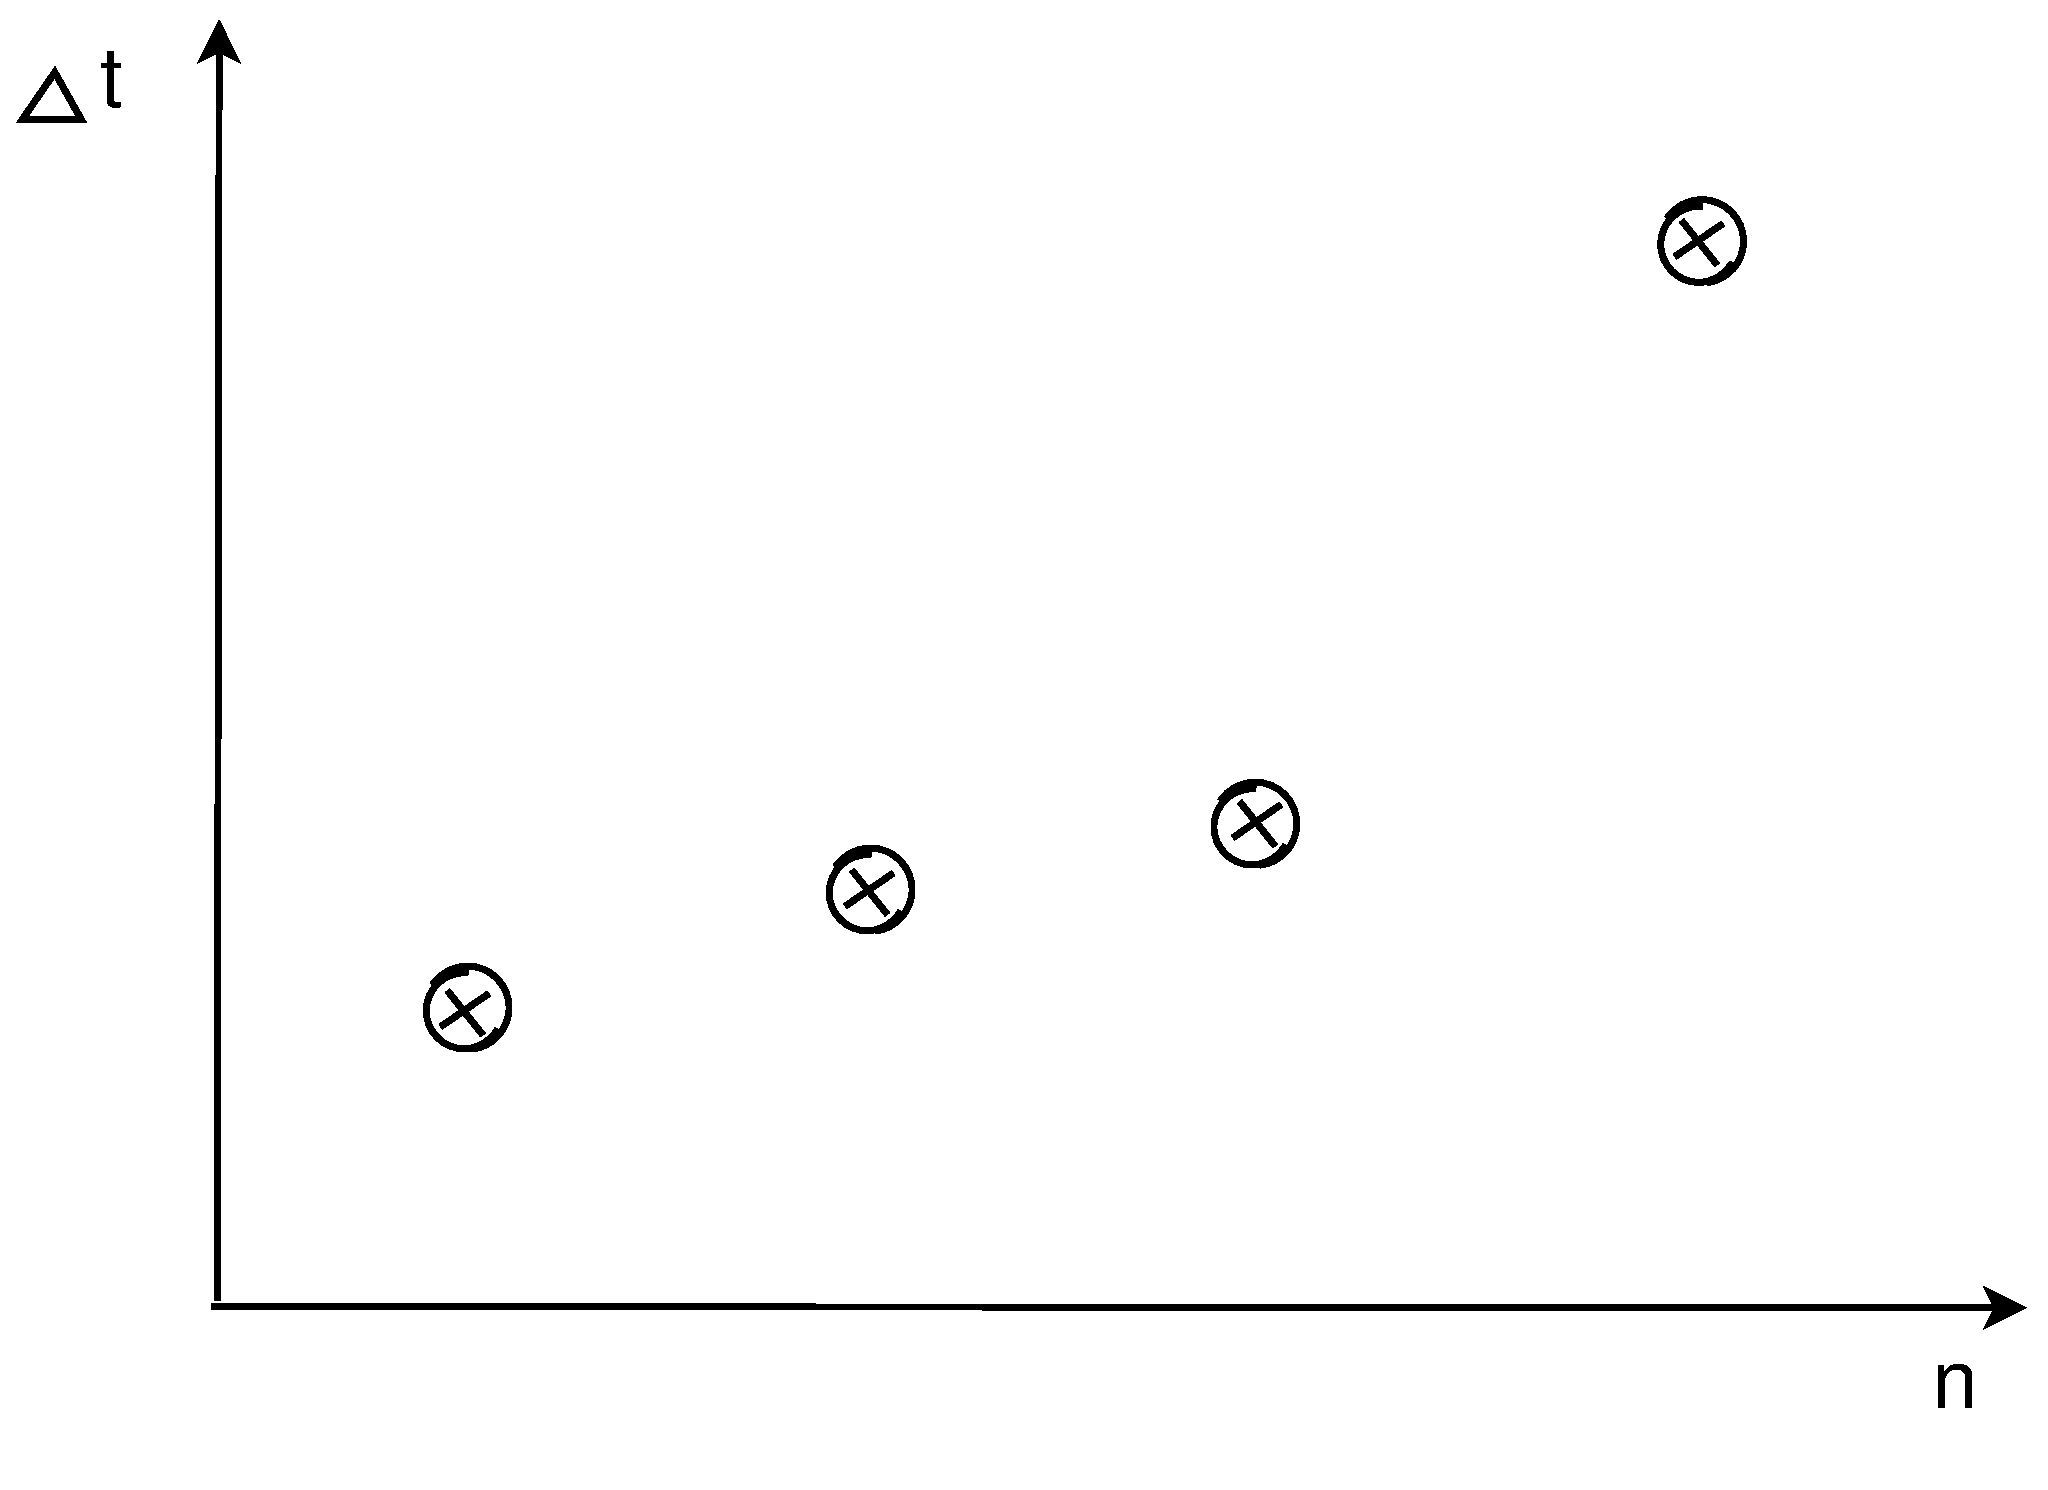
\includegraphics[width= 1\textwidth]{offset_distr}
\caption{The distribution of the phase error} \label{offset_distr}
\end{figure}
\newline One approach is
\begin{equation}
w_{ij}^{(n)} = 1 - \frac {\Delta t_{ij}^{(n)}- M^{(n)}}{\sum \Delta
t_{ij}^{(n)}-M^{(n)}}
\end{equation}
The weight is selected by the fact that the a node joining a network
should adjust its time with the network that it is joining. After
each measurement, a phase error is associated with the tabled values
to recognize how far is the sender node concerning the time that it
drifted away from the receiver node. As shown in the
$\ref{freq_defn}$, the closer the phase error is to zero, the higher
weight it is given. Thus, for a phase error of less than 9 clock
cycles, the safe region of the zone since it is in the balba of the
guard time.
\begin{center}
    \begin{tabular}{ | l | l |}
    \hline
    Phase offset & Weight \\ \hline
    0-9 cycles & 0.9 \\ \hline
    9-18 cycles & 0.7 \\ \hline
    18-29 cycles & 0.5 \\
    \hline
    \end{tabular}
\end{center}
In the calculation of the weight factor, there is another factor to
be considered here. If all the phase errors are in the upper region
which corresponds to the fact that the node is a newly joining node
to a well-established and communicating ?? network, the weight
factor of the measurments should be high if the node is wanted to
join the network. So, another step in the analaysis of the weight is
conducted to counter this effect in the hope of encountering such
claims. \newline Inorder to incorporate the effect of the
distribution of the phase errors, another quantity is introduced in
the calculation of the weight factors so that the node will adjust
its wakeup time towards the more stabilied network. Hence, the
weight factor becomes
\begin{equation}
 w_{ij} = k_i ,
\end{equation}
where $k$ represents the affiliation of the node towards the network
that the sender belongs. Hence, the connection to the network is described here.
\newline It is a two step process in which the first one describes how the nodes
are apart from each other whereas the second one describes how the node is positioned
 in the network topology which surrounds it. \newline
Thus, the next wakeup time of the node will be
\begin{equation}
t_i^{(n+1)} = t_i^{(n)} - \xi_i^{(n)} ,
\end{equation}
\begin{equation}
t_i^{(n+1)} = t_i^{(n)} - \sum_{j=0}^N{w_{ij}^{(n)}\Delta
t_{ij}^{(n)}} ,
\end{equation}
\begin{equation}
t_i^{(n+1)} = t_i^{(n)}+ SLOTTIME -
\sum_{j=0}^N{w_{ij}^{(n)}(t_i^{(n)}-t_j^{(n)})} ,
\end{equation}
\begin{equation}
t_i^{(n+1)} = t_i^{(n)} + SLOTTIME-
\sum_{j=0}^N{w_{ij}^{(n)}t_j^{(n)}} ,
\end{equation}
\begin{itemize}
 \item how to calculate the energy efficiency
 \item how to off the trail
 \item big brother
 \item effect of the speed on the nodes will be that of joining and not joining
 \item final position -> initial position to be converged in the mean time  backward movement is advised.
 \item gain factor for all algorithms
 \item different datasets for the random values
\end{itemize}
\section{Non Linear Least Square curve fitting}
Consider a set of m data points, ($x_1$, $y_1$), ($x_2$, $y_2$),$\dots$,($x_m$, $y_m$), and a curve (model function) $y=f(x, \beta)$, that in addition to the variable x also depends on n parameters,
\begin{equation}
\beta = (\beta_1, \beta_2, \dots, \beta_n),
\end{equation}
with $m\ge n$. It is desired to find the vector $\beta$ of parameters such that the curve fits best the given data in the least squares sense, that is, the sum of squares
\begin{equation}
    S=\sum_{i=1}^{m}r_i^2 ,
\end{equation}
is minimized, where the residuals (errors) $r_i$ are given by
\begin{equation}
    r_i = y_i - f(x_i,\beta)
\end{equation}
for i=1,2,$\dots$, $m$.
\newline
The minimum value of $S$ occurs when the gradient is zero. Since the model contains n parameters, there are n gradient equations:
\begin{equation}
    \frac{\partial S}{\partial \beta_j}=2\sum_i r_i\frac{\partial r_i}{\partial \beta_j}=0 \ (j=1,\ldots,n).
\end{equation}
In a non-linear system, the derivatives $\frac{\partial r_i}{\partial \beta_j}$ are functions of both the independent variable and the parameters, so these gradient equations do not have a closed solution. Instead, initial values must be chosen for the parameters. Then, the parameters are refined iteratively, that is, the values are obtained by successive approximation,
\begin{equation}
    \beta_j^{k+1}=\beta^k_j+\Delta \beta_j.
\end{equation}
Here, k is an iteration number and the vector of increments, $\Delta \beta_j$, is known as the shift vector. At each iteration, the model is linearized by approximation to a first-order Taylor series expansion about $\beta^k$!
\begin{equation}
    f(x_i,\beta)\approx f(x_i,\beta^k) +\sum_j \frac{\partial f(x_i, \beta^k)}{\partial \beta_j} \left(\beta^k_j -\beta_j \right)=f(x_i, \beta^k)+\sum_j J_{ij} \Delta\beta_j.
\end{equation}
The Jacobian, $J$, is a function of constants, the independent variable and the parameters, so it changes from one iteration to the next. Thus, in terms of the linearized model,
\begin{equation}
\frac{\partial r_i}{\partial \beta_j}=-J_{ij}
\end{equation}
and the residuals are given by
\begin{equation}
    r_i=\Delta y_i- \sum_{j=1}^{j=n} J_{ij}\Delta\beta_j \Delta y_i=y_i- f(x_i, \beta^k).
\end{equation}
Substituting these expressions into the gradient equations, they become
\begin{equation}
    \sum_{i=1}^{i=m}J_{ij} \left( \Delta y_i-\sum_{j=1}^{i=n} J_{ij}\Delta \beta_j \right)=0
\end{equation}
which, on rearrangement, become n simultaneous linear equations, the normal equations
\begin{equation}
    \sum_{i=1}^{i=m}\sum_{k=1}^{k=n} J_{ij}J_{ik}\Delta \beta_k=\sum_{i=1}^{i=m} J_{ij}\Delta y_i (j=1,n).\,
\end{equation}
The normal equations are written in matrix notation as
\begin{equation}
    \left(J^TJ\right)\Delta  \beta=J^T\Delta y
\end{equation}
When the observations are not equally reliable, a weighted sum of squares may be minimized,
\begin{equation}
    S=\sum_{i=1}^{i=m}W_{ii}r_i^2.
\end{equation}
Each element of the diagonal weight matrix, $W$ should, ideally, be equal to the reciprocal of the variance of the measurement. The normal equations are then
\begin{equation}
    \left(J^TWJ\right)\Delta  \beta=J^TW\Delta y
\end{equation}
These equations form the basis for the Gauss-Newton algorithm for a non-linear least squares problem.\newline
In linear least squares the objective function, S, is a quadratic function of the parameters.
\begin{equation}
    S=\sum_i W_{ii} \left(y_i-\sum_jX_{ij}\beta_j \right)^2
\end{equation}
When there is only one parameter The graph of S with respect to that parameter will be a parabola. With two or more parameters the contours of S with respect to any pair of parameters will be concentric ellipses (assuming that the normal equations matrix $X^TWX$ is positive definite). The minimum parameter values are to be found at the centre of the ellipses. The geometry of the general objective function can be described as paraboloid elliptical. In NLLSQ the objective function is quadratic with respect to the parameters only in a region close to its minimum value, where the truncated Taylor series is a good approximation to the model.
\begin{equation}
    S \approx\sum_i W_{ii} \left(y_i-\sum_j J_{ij}\beta_j \right)^2
\end{equation}
The more the parameter values differ from their optimal values, the
more the contours deviate from elliptical shape. A consequence of
this is that initial parameter estimates should be as close as
practicable to their (unknown!) optimal values. It also explains how
divergence can come about as the Gauss-Newton algorithm is
convergent only when the objective function is approximately
quadratic in the parameters.\newpage \section{Kalman Filter} The
kalman filter addresses the general problem of trying to estimate
the state $x$ of a discrete-time controlled process that is governed
by the linear stochastic difference equation
\begin{equation}
 x_k = Ax_{k-1} + Bu_k + w_{k-1} ,
\end{equation}
with a measurement $z$ that is
\begin{equation}
 z_k = Hx_k + v_k.
\end{equation}
The random variables $w_k$ and $v_k$ represent the process and measurement noise(respectively). They are assumed to be independent(of each other), white, and with normal probability disributions
\begin{equation}
 p(w) ~N(0,Q),
\end{equation}
\begin{equation}
 p(w)~N(0,R).
\end{equation}
In practice, the process noise covariance Q and measurement noise
covariance R matrices might change with each time step or
measurement, however here we assume they are constant.\newline The
nxn matrix A in the difference equation $\ref{tdma}$ relates the
state at the previous time step k-1 to the state at the current step
k, in the absence of either a driving function or process noise.
Notethat in practice A might change with each time step, but here we
assume it is constant. The nxl matrix B realters the optional
control input $u$ to the state x. The mxn matrix H in the
measurement equation $d$ realters the state to the measurement
$z_k$. In practice H might change with each time step or
measurement, but here we assume it is constant.\newline {The
algorithm} The Kalman filter estimates a process by using a form of
feedback control: the filter estimates the process state at some
time and then obtains feedback in the form of (noisy) measurements.
As such, the equations for the Kalman filter fall into two groups:
time update equations and measurement update equations. The time
update equations are responsible for projecting forward (in time)
the current state and error covariance estimates to obtain the a
priori estimates for the next time step. The measurement update
equations are responsible for the feedbacks i.e. for incorporating a
new measurement into the a priori estimate to obtain an improved a
posteriori estimate. The time update equations can also be thought
of as predictor equations, while the measurement update equations
can be thought of as corrector equations.
\newline
We define $x_k  R$ to be our a priori state estimate at step k given
knowledge of the process prior to step k, and $x_k ∈ R$ to be our
a posteriori state estimate at step k given measurement $z_k$ . We
can then define a priori and a posteriori estimate errors as
\begin{equation}
e_k = x_k  x_k ,
\end{equation}
\begin{equation}
e_k = x_k  x_k
\end{equation}
The a priori estimate error covariance is then
\begin{equation}
P_k = E[ e_k e_k ]
\end{equation}
and the a posteriori estimate error covariance is
\begin{equation}
P_k = E[e_k e_k]
\end{equation}
In deriving the equations for the Kalman filter, we begin with the goal of finding
an equation that computes an a posteriori state estimate as a linear
combination of an a priori estimate and a weighted difference
between an actual measurement and a measurement prediction as shown
below in equation $\ref{eq:diff}$.
\begin{equation}
\tilde x_k = \tilde x_k + K(z_k-H\tilde x_k) \label{diff}
\end{equation} The
difference $z_k - H\tilde x_k$ in equation $\ref{eq:diff}$is called
the the residual. The residual reflects the discrepancy between the
predicted measurement $H\tilde x_k$ and the actual measurement
$z_k$. A residual of zero means that the two are in complete
agreement. \newline The $nxm$ matrix K in equation $\ref{eq:Kaga}$
is chosen to be the gain or blending factor that minimizes the a
posteriori error covariance equation $\ref{eq:cov}$. This
minimization can be accomplish ed by first substituting equation
$\ref{eq:cov}$ into the above definition for , substituting that
into equation $\ref{eq:kal}$, performing the indicated expectations,
taking the derivative of the trace of the result with respect to K,
setting that result equal to zero, and then solving for K. $Details
for refrence$. One form of the resulting K that minimizes equation
$\ref{eq:cov}$ is given by
\begin{equation}
K_k = P_kH^{T}(HP_kH^{T} + R)^{-1}\end{equation}\begin{equation}
    = \frac{P_kH^T}{HP_kH^T + R}
\end{equation}
Looking at equation $\ref{eq:above}$, we see that as the measurement
error covariance $R$ approaches zero, the gain K weights the
residual more heavily. Specifically,
\begin{equation}
\mathop {\lim }\limits_{R_k \to 0 } {K_k} = H^{-1}.
\end{equation}
On the other hand, as the a priori estimate error covariance $P_k$
approaches zero, the gain K weights the residual less heavily.
Specifically,
\begin{equation}
\mathop {\lim }\limits_{P_k \to 0 } {K_k} = 0.
\end{equation}
In the selection of the matrices, we will consider different
situations of the WSN. The coefficient matrix is used to project the
estimated value of the node wakeup time and the received time of the
neighbors, in an increasing order. Hence, to tackle the scenarios of
node appearance and disappearance, the new node joining the network
should be synchronized with the already established "status quo" of
the network.\newline The previous offset that is applied to the node
in order to adjust the wakeup time of the nodes can be used as a
starting point for the current wakeup time calculation. Logical
thinking suggest that with the stable network where the nodes remain
intact, the wakeup time of the node is expect to be the same despite
the clock drift( citation needed). So, the initial value of the
estimated value of the wakeup time is taken from the previous value,
with a factor of $p$ which represents the wakeup time of the
neighboring nodes, which has also been changed in the mean
time.(citation needed).
In the filter design, the covariance matrices play a significant role in the
overall implementation of the algorithm. In which case, the constants tell which
design philosophy is that we are taking. \newline
\begin{figure}
\centering
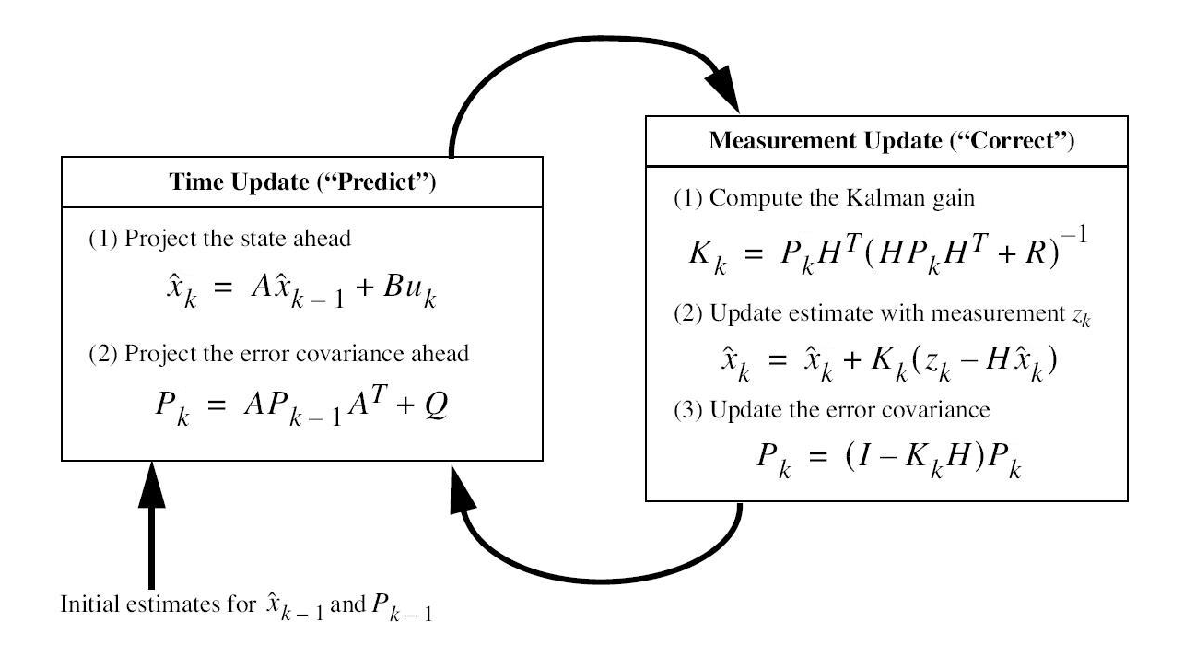
\includegraphics[width=0.8\textwidth]{kalman_update}
\caption{Kalman filter algorithm}
\end{figure}
Thus, the update equations are applied in the series of measurement
to end up in an optimal(next time) wakeup time of the node.\newline
The covariance matrices $R$ and $Q$ have their own significance. R
represents how we value the measured values to affect the result of
the outcome. And $Q$ sends a signal as to how we have to evaluate
the estimated value.\newline Analysis: The estimated values, which
base on a stable background ... are more prone to be write after a
series of firings. On the contrary, the measured values have large
deviations and excit... that more of the weight is going to the
estimated values.\begin{itemize}
\item Believe in Self
\item Believe in Group
\item Believe in Outsiders
\end{itemize}
\newpage
\chapter{Results and Discussion}
\section{Simulation setup}
In this chapter, the simulation setup is given which is used for
exploring the relation between the MACs. First, the MiXiM framework
is described. After that, a closer inspection will be done of the
several MAC configurations. Then, the different node configurations
are given in terms of: number of neighbors, placement, and radio
range.A separate study is being done concurrently, which researches
on the G-Mac protocol. In this research, the assumption can be made
that the slots are allocated. As G-MAC was modeled for the MyriaNed
platform, the radio is modeled very close to the official hardware.
It is running in the 2.4GHz band at a speed of 2Mbps. The more
factors that influence the simulation, the harder it is to interpret
the results. A Discrete Event Simulator (DES) will break down a
simulation into discrete chunks. Every event will occur at some
countable time moment and will be given in chronological order. The
advantage of this distinction is two-fold. First, simulations will
not be dependant on some real-time clock. Second, events can be
isolated to perform certain measurements.
\newline One such DES is called OMNeT++. It provides a component architecture for models.
Components are programmed in C++, then assembled into larger
components and models using a high-level language. These components
were merged into a joined simulation effort by several academic
institutes around Europe: MiXiM. It is specialized on wireless
sensor networks. Nodes are modeled as a set of separate components
stacked upon each other, as shown in Figure $osimodel$.
\begin{figure}
\centering
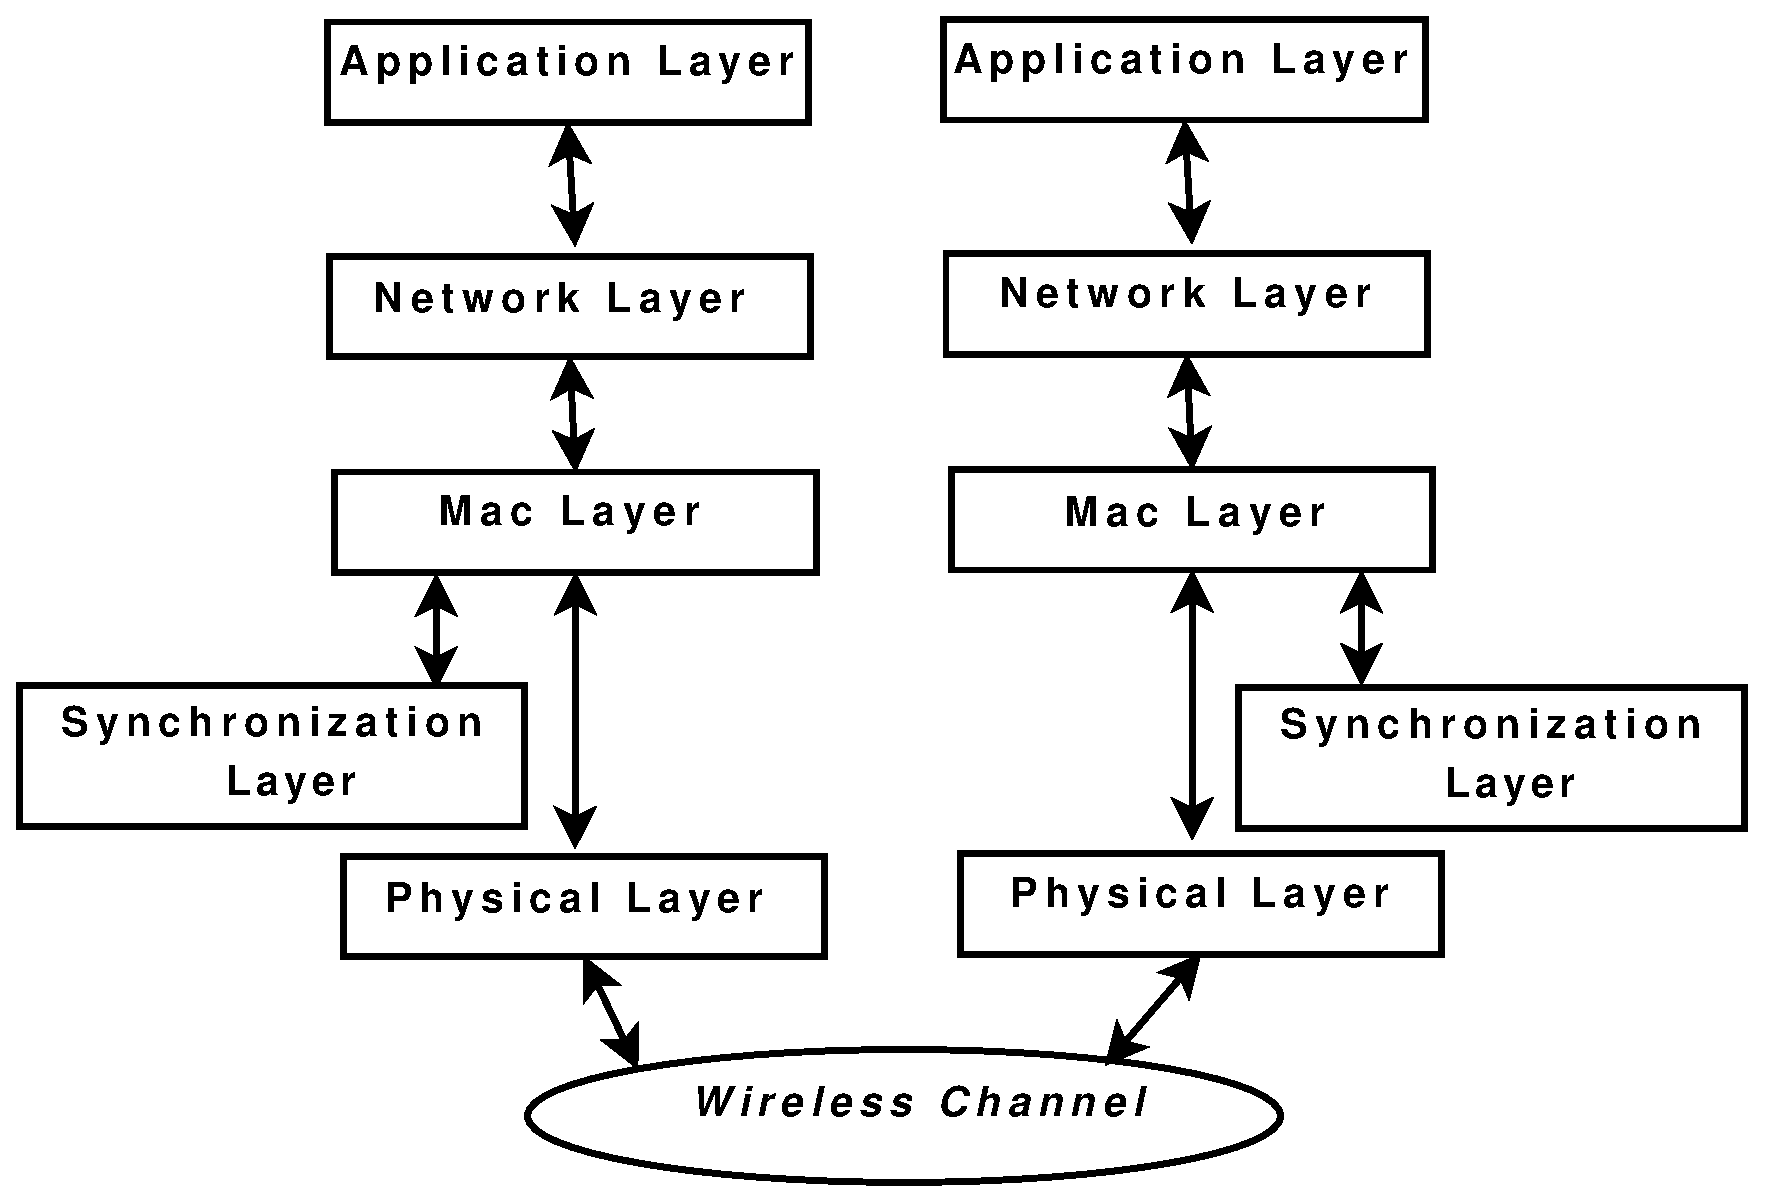
\includegraphics[width=1\textwidth]{osimodel}
\caption{Mixim Nodes} \ label{osimodel}
\end{figure}
The synchronization is done as a separate layer. The communication
over the channels is done in a unidisc way. All nodes in range of
the radio actually receive the data, those that are outside are
excluded.\newline The simulation environment is used. In the
simulation, the field in which the nodes are deployed in the sensor
field of the 100 m by 100m. The number of nodes is varied for the
different simulation cases. The dynamicity of the nodes is taken
from the static to the full speed case. In the simulation, the
channel is taken as a specific wirless channel model, with the
attenuation constant of $\gamma = 2.5$. The shadowing variance of
the channel is taken to be in the range of the timing so that more
and more time is taken to be given:
\begin{center}
    \begin{tabular}{ | l | l |}
    \hline
    Number of active slots & 990 \\ \hline
    Duration time frame & 1s \\ \hline
    Network Discovery rate & 1 per time frame \\ \hline
    Busy slot listening & 1 per 32 time frame \\ \hline
    Field area & 100 x 100 \\ \hline
    Duty Cycle & 1$\%$ \\ \hline
    \end{tabular}
\end{center}
\section{Computer simulation Results}
\begin{itemize}
\item Simulation : Speed 0 x2 , Speed 100 x2 , speed walking x2
\item Measured : median vs t , kalman vs t , weight vs t ,
\item guard time vs energy expenditure
\end{itemize}
\begin{figure}
\centering
\begin{tabular}{cc}
\epsfig{file=output.eps,width=0.5\linewidth,clip=} &
\epsfig{file=output2.eps,width=0.5\linewidth,clip=} \\
\epsfig{file=output3.eps,width=0.5\linewidth,clip=} &
\epsfig{file=output4.eps,width=0.5\linewidth,clip=}
\end{tabular}
\end{figure}
\begin{figure}
\centering
\begin{tabular}{cc}
\epsfig{file=output4.eps,width=0.5\linewidth,clip=} &
\epsfig{file=output5.eps,width=0.5\linewidth,clip=} \\
\epsfig{file=output6.eps,width=0.5\linewidth,clip=} &
\epsfig{file=output4.eps,width=0.5\linewidth,clip=}
\end{tabular}
\end{figure}
\section{Energy Consumption and Guard time tradeoff}
\newpage
\chapter{Conclusion and Recommendation}
\begin{itemize}
\item Guard time calculation
\item Trade off in calculation
\item 270 microsecond
\item practical implementation - median is fine working
\item sensor addition
\item median - to be the best
\end{itemize}
Recommendation
\begin{itemize}
\item Integration with the Mac protocol
\item Frequency adjustment
\item temperature sensor
\end{itemize}
\subsection*{Acknowledgment}
\newpage
\begin{thebibliography}{References}
\bibitem{1} Mirollo,R. and Strogatz,S. , Synchronization of pulse-coupled biological oscillators, SIAM J. Appl. Math, vol. 50, no. 6, pp. 1645-1662,Dec 1990.
\bibitem{2} Romer,K. Time Synchronization in Ad Hoc Networks. In: Proceedings of the Second ACM International Symposium on Mobile Ad Hoc Networking and Computing, Long Beach, California. 2001
\bibitem{3} Holger Karl and A.Willig , Protocols and Architectures for Wireless Sensor Networks , Wiley,July 2006.
\bibitem{4} C. Cordeiro and D. Agrawal , Ad hoc and Sensor Networks Theory and applications , World Scientific Publishing, 2006.
\bibitem{5} F. Zhao and L. Guibas , Wireless Sensor Networks: an Information Processing approach , Elsevier , 2004.
\bibitem{6} Fan, R., Lynch, N.: Gradient clock synchronization. In: Proceedings of the 23rd ACM Symposium on Principles of Distributed Computing (PODC004),
St. John's, Newfoundland, Canada, July 2004, pp. 3200327. ACM Press,
New York 2004.
\bibitem{7}Romer, K.: Time synchronization in ad hoc networks. In: Proceedings of the 2nd ACM International Symposium on Mobile Ad Hoc Networking and
Computing (MOBIHOC001), Long Beach, CA, USA, October 2001, pp.
173082. ACM Press, New York 2001.
\bibitem{8} Elson, J., Girod, L., Estrin, D.: Fine-grained network time synchronization using reference broadcasts. Proceedings of the 5th Symposium on
Operating Systems Design and Implementation (OSDI002)
36(SI),1470163,2002.
\bibitem{9} S. PalChaudhuri, A.K. Saha, and D.B. Johnson, Adaptive Clock Synchronization in Sensor Networks, Information Processing in Sensor Networks (ISPN), Apr. 2004.
\bibitem{10}Tjoa, R., and et al. Clock Drift Reduction For Relative Time Slot TDMA-Based Sensor Networks, 15th IEEE International Symposium on Personal, Indoor and
Mobile Radio Communications, vol. 2, pp. 1042-1047, 5-8 Sept. 2004.
\bibitem{12} Yang, Q., and et al. A Decentralized Slot Synchronization Algorithm for TDMA-Based Ad Hoc
Networks.
\bibitem{13} Werner-Allen, G. and et al , Firefly-inspired sensor network synchronicity with realistic radio effects, Proceedings of the 3rd international
conference on Embedded networked sensor systems,, San Diego,
California, November 02-04, 2005.
\bibitem{14} Yang,Q. and Shi,J. An interference elimination method for decentralized slot synchronization in TDMA-based wireless ad hoc network.
\bibitem{15} Fault-Tolerant Cluster-Wise Clock Synchronization for Wireless Sensor Networks.
\bibitem{16} FTSP - Flooding Time Synchronization Protocol.
\bibitem{17} Romer,K. Time Synchronization in Ad Hoc Networks.
\bibitem{18} Zhong Xiaofeng, Wang youzheng, etc, Synchronization in TDMA Ad Hoc Networks, Proceedings of IEEE Vehicular Technology Conference, 2004, pp.5011-5014, 2004.
\bibitem{19} Jeremy Elson and Deborah Estrin. Time Synchronization for Wireless Sensor Networks. In Proceedings of the 15th International
Parallel and Distributed Processing Symposium (IPDPS-01). IEEE
Computer Society, April 23-27 2001.
\end{thebibliography}
\appendix
\chapter{Myrianed Node v2.0}
\chapter{32KHz Crystal clock Datasheet}
\chapter{ATmega128}
\end{document}
